\documentclass[]{article} 
\usepackage{proceed2e}
\usepackage{subfigure}
\usepackage[numbers,sort]{natbib}
\usepackage{amsmath}
\usepackage{amssymb}
\usepackage{graphicx}
\usepackage{ifthen,version}
\newboolean{include-notes}
\usepackage{algorithm}
\usepackage{algpseudocode}
%\usepackage{adjustbox}
\usepackage[usenames,dvipsnames]{color}
\newcommand{\stnote}[1]{\textcolor{Blue}{\textbf{ST: #1}}}
\newcommand{\jmnote}[1]{\textcolor{Green}{\textbf{JM: #1}}}
\newcommand{\dnote}[1]{\textcolor{Orange}{\textbf{D: #1}}}
\newcommand{\gnote}[1]{\textcolor{Red}{\textbf{G: #1}}}


\title{Affordance-Aware Planning}

\begin{document}
\author{}
\maketitle

\begin{abstract}
%Current methods for decision-making under uncertainty require
%exhaustive enumeration of all possible states and actions, leading to
%exponential run times caused by 

Planning algorithms for non-deterministic domains are often
intractable in large state spaces due to the well-known ``curse of
dimensionality.''  Existing approaches to address this problem fail to
prevent the system from considering many actions which would be
obviously irrelevant to a human solving the same problem.  We
introduce a novel, state- and reward- general approach to limiting the
branching factor in large domains by encoding knowledge about the
domain in terms of {\em affordances}~\citep{gibson77}.  Our affordance
formalism can be coupled with a variety of planning frameworks to
create ``affordance-aware planning,'' allowing an agent to efficiently
prune its action space based on domain knowledge and its current
subgoal.  This pruning significantly reduces the number of
state/action pairs the agent needs to evaluate in order to act
optimally. We demonstrate our approach in the Minecraft domain,
showing significant increase in speed and reduction in state-space
exploration compared to the standard versions of these algorithms.

% options, and macro actions
\end{abstract}

%\stnote{High level things we should add:
%\begin{itemize}
%\item Runtime of the three algorithms in big O notation.
%\item Results with non-deterministic T.
%\end{itemize}
%}

\section{INTRODUCTION}

As robots move out of the lab and into the real world, planning
algorithms need to scale to domains of increased noise, size, and
complexity.  A classic formalization of this problem is a stochastic
sequential decision making problem in which the agent must find a
policy (a mapping from states to actions) for some subset of the state
space that enables the agent to achieve a goal from some initial
state, while minimizing any costs along the way.
%A classic formalization of this issue is the
%sequential decision making problem, where 
Increases in planning problem size
and complexity directly correspond to an explosion in the state-action
space. Current approaches to solving sequential decision making
problems in the face of uncertainty cannot tackle these problems 
as the state-action space becomes too large~\citep{grounds05}.

To address this state-space explosion, prior work has explored adding
knowledge to the planner to enable it to solve problems in these
massive domains, such as options~\citep{sutton99} and
macroactions~\citep{Botea:2005kx,Newton:2005vn}. However, these
approaches add knowledge in the form of additional high-level actions
to the agent, which {\em increases} the size of the state/action space
(while also allowing the agent to search more deeply within the
space).  The resulting augmented space is even larger, which can have
the paradoxical effect of increasing the search time for a good
policy.

\begin{figure}
\centering
%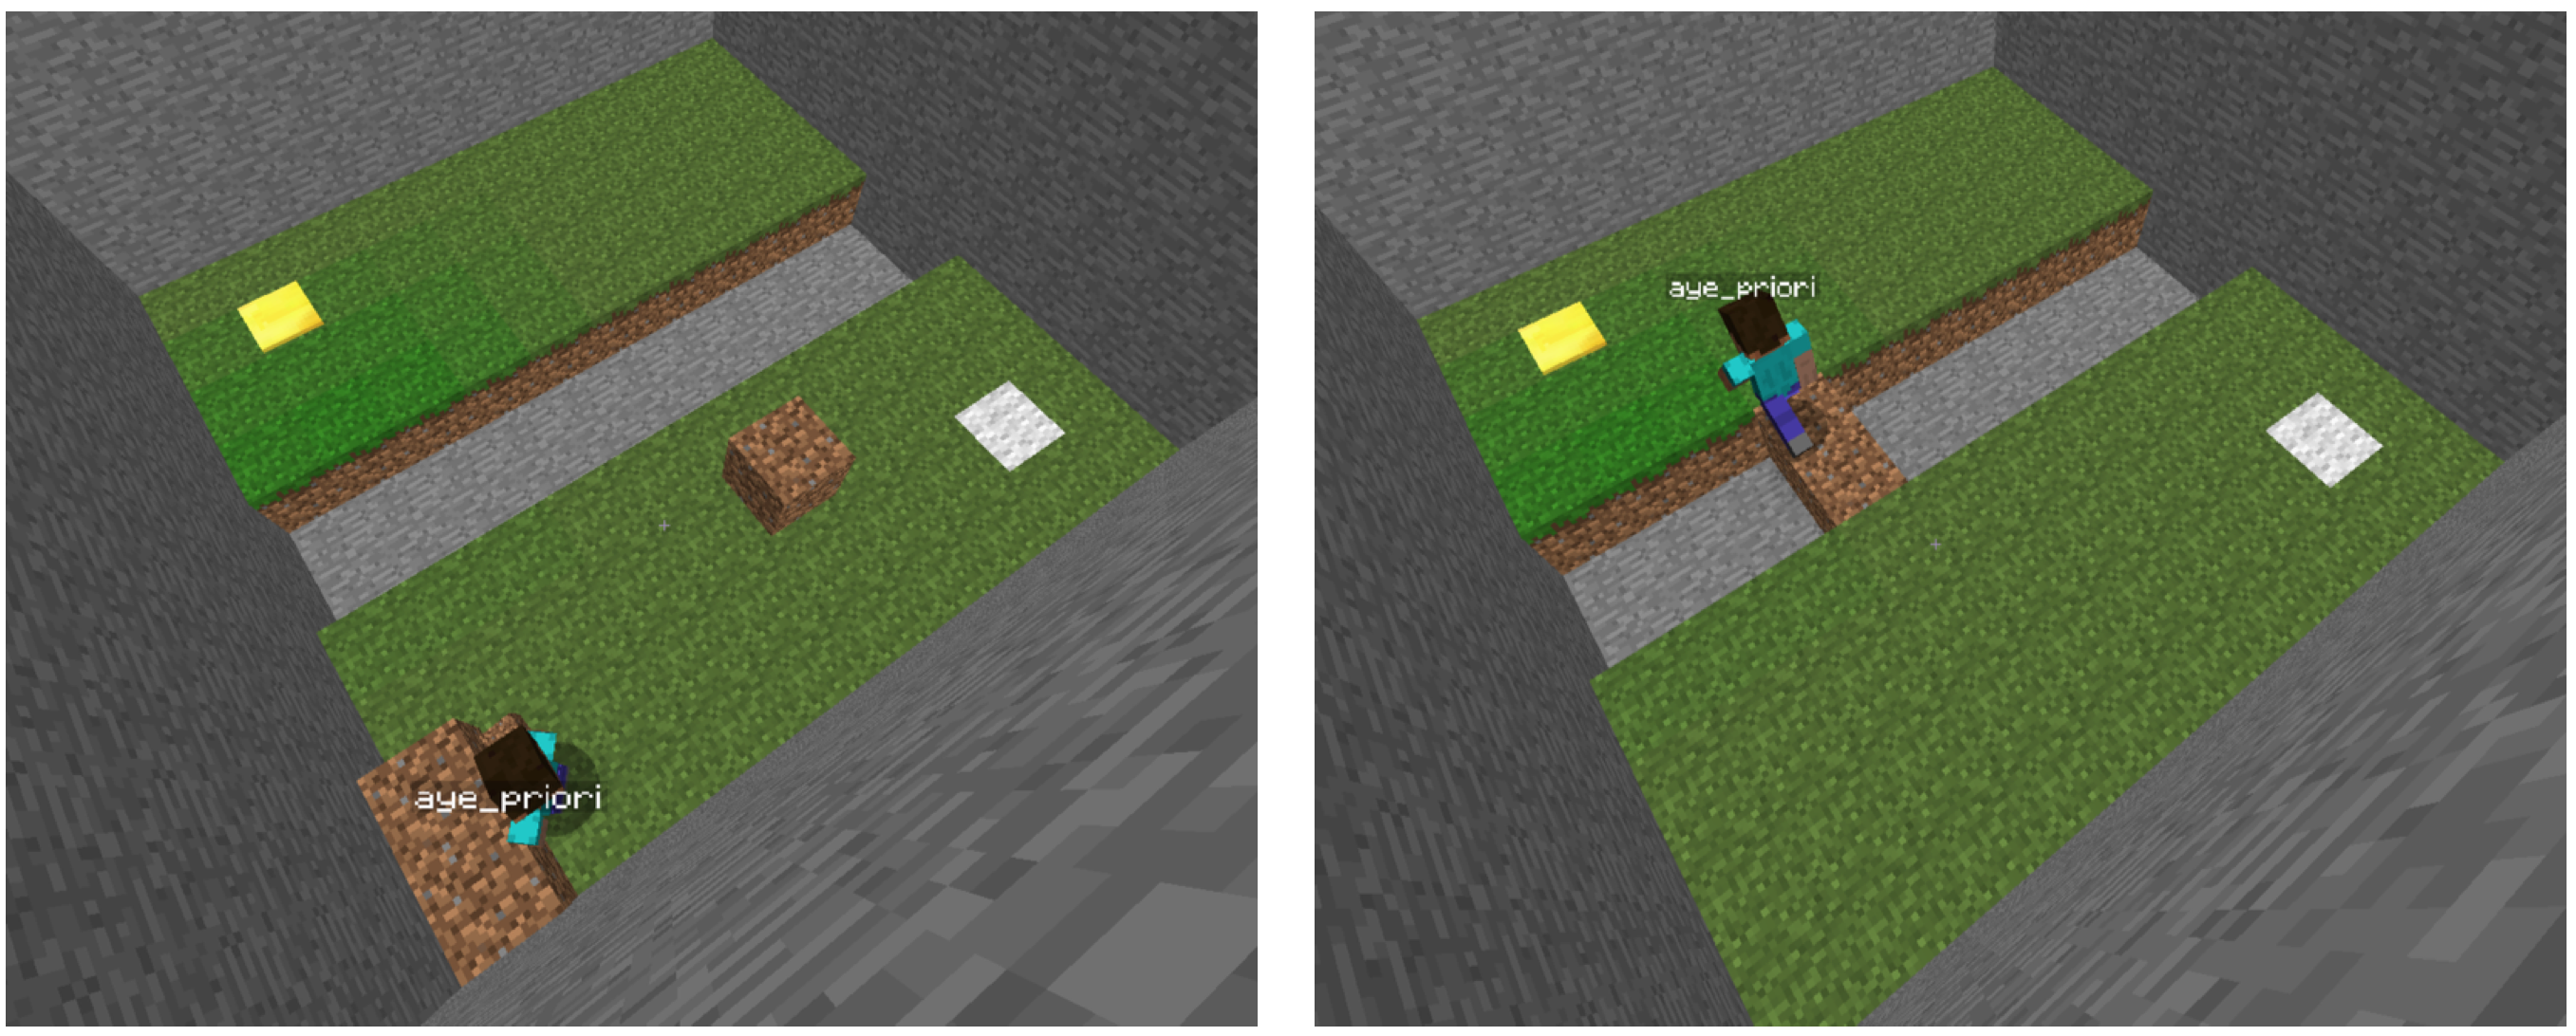
\includegraphics[scale=0.18]{figures/bridgeworld_vi_vs_aff.png}
\subfigure[Planning with VI.]{
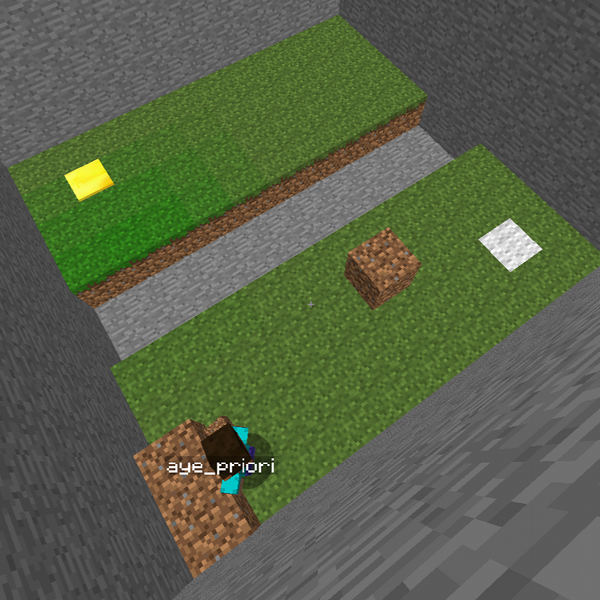
\includegraphics[width=0.5\linewidth]{figures/fig_1_vi_cropped.png}}%
\subfigure[Planning with affordances.]{
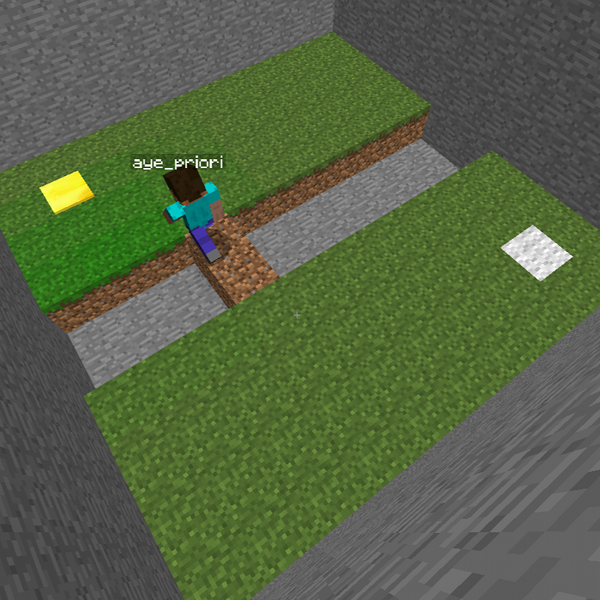
\includegraphics[width=0.5\linewidth]{figures/fig_1_aff_cropped.png}}%
  \caption{Scenes from a Minecraft agent planning using Value
    Iteration (VI) compared to affordance-aware VI in a bridge
    building task; the start is in the white square, and the goal is
    the yellow square.  VI considers states which would be obviously
    irrelevant to a human solving the same problem, such as stacking
    blocks in the corner.  Our affordance agent, in contrast, focuses
    on placing blocks in the trench, which are much more relevant to
    reaching the goal.\label{fig:minecraft}}
\end{figure}

Instead, we propose a formalism that enables an agent to focus on
problem-specific aspects of the environment, guiding the search toward
the most relevant and useful parts of the state-action space.  This
approach reduces the size of the explored state action space, leading
to dramatic speedups in planning.  Our approach is a formalization of
{\em affordances}, introduced by \citet{gibson77} as ``what [the
  environment] offers [an] animal, what [the environment] provides or
furnishes, either for good or ill.''
      
      We formalize the notion of an affordance as a piece of planning
      knowledge provided to an agent operating in a Markov Decision
      Process (MDP). We explain how affordances can be leveraged by a
      variety of planning algorithms to prune the action set the agent
      uses dynamically based on the agent's current goal.  We call any
      planning algorithm that uses affordances to prune the action set
      an {\it affordance-aware} planning algorithm.  Affordances are
      not specific to a particular reward function or state space, and thus,
      provide the agent with transferable knowledge that is effective
      in a wide variety of problems. Because affordances
      define the {\em kind} of goals for which actions are useful,
      affordances also enable high-level reasoning that can
      be combined with approaches like subgoal planning for even
      greater performance gains. In Figure \ref{fig:epicworld}, we demonstrate the effectiveness of
      affordance-aware subgoal planning on a complicated task
      in the Minecraft domain - a video is provided of the agent achieving this task \footnote{Watch at: https://vimeo.com/88689171}.
      We let other standard planners try to solve this task for several hours, but they all failed
      to converge on a policy (while affordance-aware subgoal planner found a near-optimal
      policy in less than 5 minutes).


%~\citep{kaelbling99} -- (JM: I don't think you should cite this. This paper involves
%partially observable markov decision processes, which this work does not evaluate.)

%We demonstrate that, like
%an option or macro-action, an affordance provides additional
%information to the agent, enabling more transferable and efficient
%planning.  However, unlike previous approaches, an affordance enables
%more significant speedups by reducing the branching-factor of
%the search space, enabling an agent to focus its search on the most
%relevant part of the problem at hand.  This approach means that a
%single set of affordances provides general domain knowledge, becoming
%relevant just when the agent reasons that it needs to pursue a
%particular goal.  Furthermore, affordances are not specific to a
%particular reward function or goal, and thus, provide the agent with
%transferrable knowledge that is effective in a wide variety of
%problems.


\section{Minecraft Domain}
We use Minecraft as our planning and evaluation domain. Minecraft is a
3-D blocks world game in which the user can place and destroy blocks
of different types.  Minecraft players have constructed complex
worlds, including models of a scientific graphing
calculator~\footnote{https://www.youtube.com/watch?v=wgJfVRhotlQ};
scenes from a Minecraft world appear in Figure~\ref{fig:minecraft}.  

% Stochasticity paragraph
Minecraft serves as an effective parallel for the actual world, both
in terms of approximating the complexity and scope of planning
problems, as well as modeling the uncertainty and noise presented to a
real world agent.  For instance, robotic agents are prone to
uncertainty all throughout their system, including noise in their
sensors (cameras, LIDAR, microphones, etc.), odometry, control, and
actuation.  In order to accurately capture some of the inherent
difficulties of planning under uncertainty, the Minecraft agent's
actions were modified to have stochastic outcomes. These stochastic
outcomes may require important changes in the optimal policy in
contrast to deterministic actions, such as keeping the agent's
distance from a pit of lava.


 Although we made the actions of the Minecraft domain stochastic, we have chosen to give the Minecraft agent non-noisy sensory
data about the Minecraft world, as vision is assumed to be outside the scope of this
project.

%One of the difficulties of planning in a noisy world 
%is that unintended consequences can lead to disastrous results. A robotic agent,
%for instance, may unintentionally move its arm into a wall, damaging the wall or the robot itself. We
%model these potentially dangerous situations by requiring that the actions in the
%Minecraft domain be non-deterministic, and place pits of lava in many (but not all)
%of our experiments, which force the agent to plan conservatively in order to avoid
%falling in. This is intended to model the conservative nature of planning with a stochastic and potentially
%dangerous agent acting in the real world, such as a robot.

As a running example, we will consider the problem of an agent
attempting to cross a trench in a $4 \times 4 \times 2$ Minecraft
world; a schematic appears in Figure~\ref{fig:bridgeworld}. The floor
(at $z = 1)$\footnote{The $z$-axis is the height of the Minecraft
  world. Similarly, the $x$-axis is its width and the $y$-axis is its
  length.} is composed of 8 solid blocks, with horizontal empty
trenches at $y = 2$ and $y = 3$. The agent is at the starting location
$(1, 1, 2)$ and needs to reach the goal at $(4,4,2)$

\begin{figure}
\centering
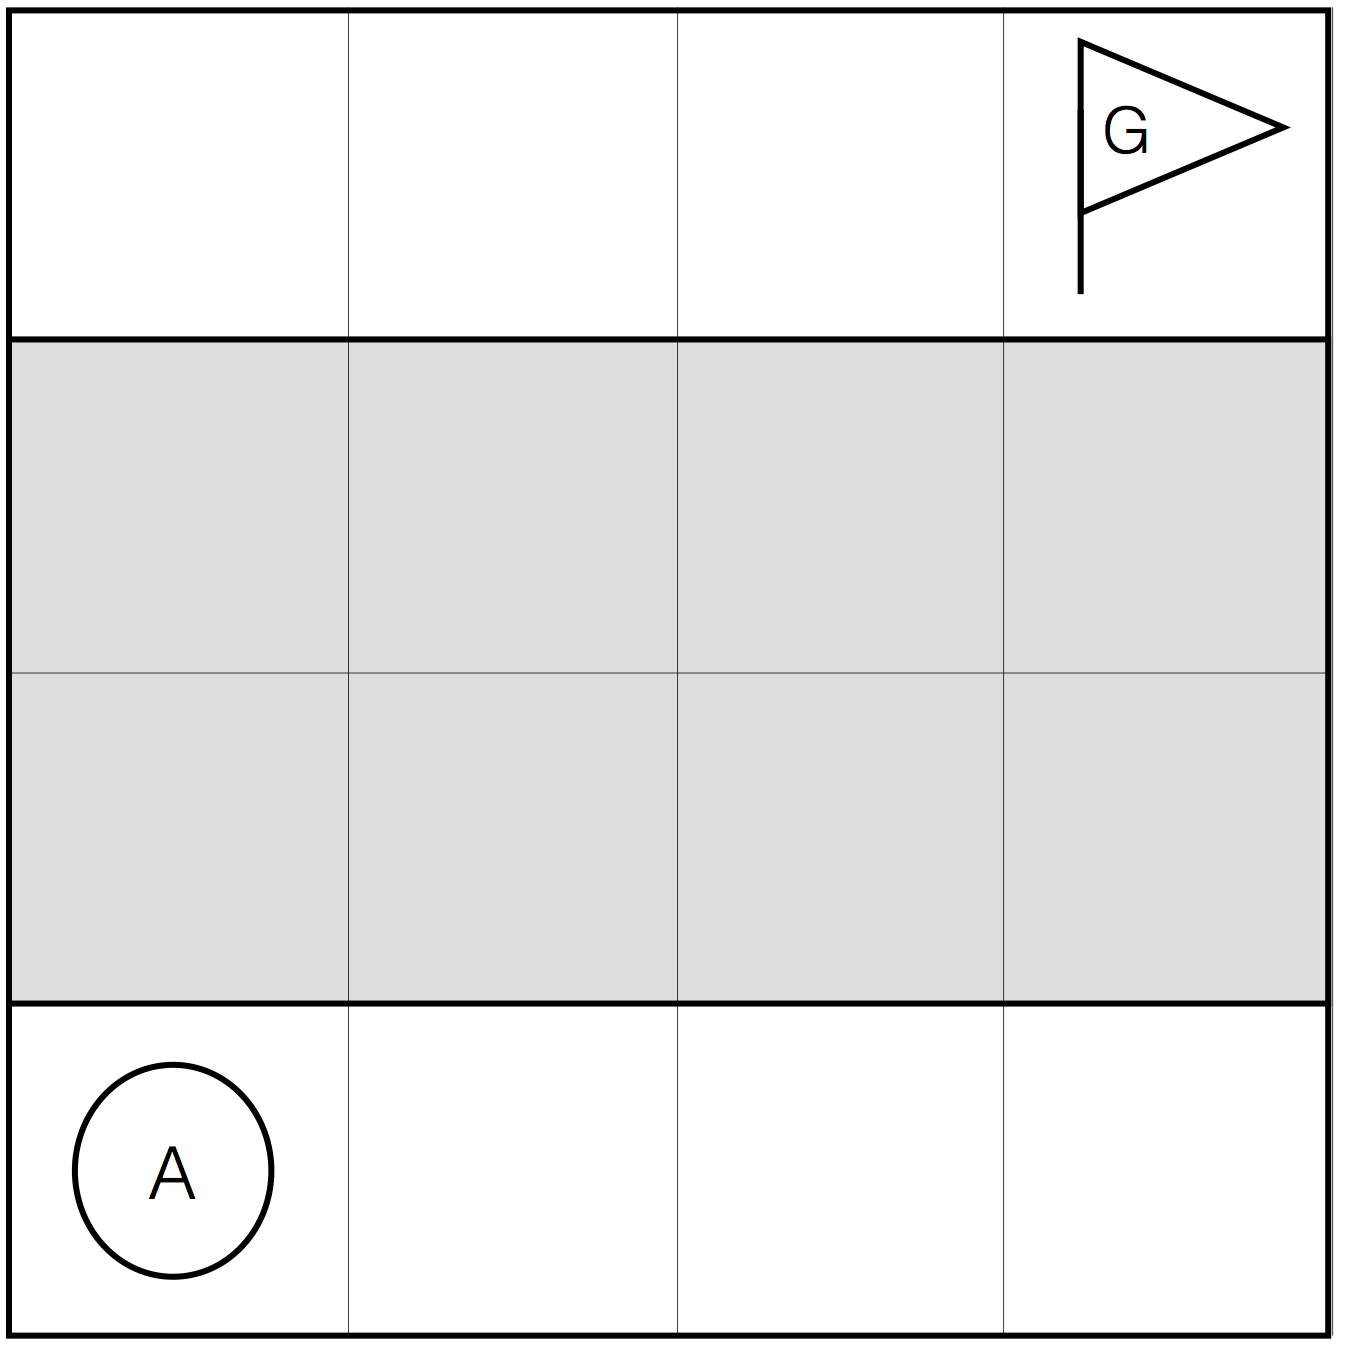
\includegraphics[scale=0.2]{figures/bridgeworld.png}
\caption{\texttt{BRIDGEWORLD},
\label{fig:bridgeworld}}
\end{figure}

To solve the problem, the agent must place a block in the trench to
form a bridge, then cross the bridge to reach the goal.  This task is
challenging for planning algorithms to solve because the reachable
state space in Minecraft is so large. For example, the number of
locations an agent can place and destroy blocks alone can result in a
combinatorial explosion of the state space. An affordance-aware
planner, however, (when equipped with the proper affordances) will
only consider placing or destroyin a block when it that action moves
the agent closer to its goal. Thus, when the agent is in state in
which block placement is not considered useful, the agent will not
have access to the block placement action (and will not be able to
explore the states that result in applying the block placement action
in its current state). As a result, the agent dramatically prunes its
effective action space.


%% Given an agent capable of
%% placing and destroying blocks in a world with dimensions $w \times l
%% \times h$, there are:
%% \begin{align}
%% O\left(\sum_{n=1}^{w \cdot l \cdot h} \binom{w \cdot l \cdot h}{n}\right)
%% \label{eq:mc_explode}
%% \end{align}
%% states, which is too large for a standard planner to explore in a
%% reasonable time.


%However, when running an uninformed planning
%technique such as value iteration, the agent must enumerate all
%possible states, such as placing a block in the corner and
%subsequently destroying it.  Considering these actions (which are
%obviously irrelevant to a human player) results in a combinatoric
%explosion of the state space (see Equation \ref{eq:mc_explode}).


\section{BACKGROUND}

Re review

\subsection{Affordances}

The term ``Affordance'' was introduced by \citet{gibson77}. At a
high-level, an affordance may be thought of as the
action-possibilities that an environment presents to an agent. More
specifically, Gibson proposed that an affordance be thought of as
``what [the environment] offers [an] animal, what [the environment]
provides or furnishes, either for good or ill'' ~\citep{gibson77}. He
added that an affordance may not be thought of as a physical property
of the environment itself, as an affordance must be defined with
respect to the capabilities and features of a specific animal in
addition to the environment.  There have been many attempts at
properly grounding affordances in a variety of academic
disciplines~\citep{1,2,3}. Even amongst the psychological literature
there is no clear consensus on what to make of an
affordance~\citep{oliverxx}.  The result is a landscape of academic
work that spans from psychological and cognitive science literature,
to HCI and design, to Robotics and Planning, that is largely
inconsistent about what is meant by the term {\it affordance}.  Our
aim in this paper is to provide a simple, yet general definition of an
affordance in terms of knowledge added to an MDP which enables
dramatic speedups in planning times, depending on the agent's goal.
Specifically, we define an affordance in terms of the agent's current
goal; depending on the needs of the agent, it may only perceive
certain affordances. For instance, a rock may serve as a fantastic
paper-weight to an agent seeking to weigh down a stack of papers. If
the agent's goal changes and is instead looking for a means of
propping a door open, then the agent may also perceive that the rock
will serve as an adequate doorstop.

%% The term is rich with potential,
%% but due to the body of existing work, any project whose aim is to {\it
%%   use} the concept of affordances must begin by clearly defining what
%% exactly is meant by an affordance.


%% This poses a serious problem for
%% modeling affordances, as the combination of an agent with an
%% environment (in our case, the Minecraft domain) would inevitably
%% present the agent with uncountably many affordances (i.e. consider all
%% action-possibilities for a rock in an office, or a pocket knife in a
%% kitchen). To solve this issue, we chose to encode the current needs of
%% the agent directly into each affordance. In this way, if the agent is
%% seeking to prop open a door, then the agent's action possibilities for
%% doing so are reduced to using a rock, a brick, a weight, a rubber
%% wedge, and so on. This allows for robust definitions of affordances
%% that do not require an extensive enumeration of all
%% action-possibilities of a given agent in an environment. Instead, our
%% model of affordances only refers to action-possibilities that are
%% useful to an agent when it is trying to achieve a certain type of
%% goal.

% by our reading, an affordance consists of a perceiving, autonomous {\it agent} in an {\it environment} (which we model with an OO-MDP), along with a {\it goal} that the agent is trying to achieve (a lifted goal description). This take on affordances may be thought of as from the {\it agent's} perspective.

\subsection{OO-MDP}

We define affordances in terms of propositional functions on states. Our definition builds on the Object-Oriented Markov Decision Process
(OO-MDP)~\citep{diuk08}.  OO-MDPs are an extension of
the classic Markov Decision Process (MDP).  A classic MDP is a
five-tuple: $\langle \mathcal{S}, \mathcal{A}, \mathcal{T},
\mathcal{R}, \gamma \rangle$, where $\mathcal{S}$ is a state-space;
$\mathcal{A}$ is the agent's set of actions; $\mathcal{T}$ denotes
$\mathcal{T}(s' \mid s,a)$, the transition probability of an agent
applying action $a \in \mathcal{A}$ in state $s \in \mathcal{S}$ and
arriving in $s' \in \mathcal{S}$; $\mathcal{R}(s,a,s')$ denotes the
reward received by the agent for applying action $a$ in state $s$ and
and transitioning to state $s'$; and $\gamma \in [0, 1)$ is a discount
  factor that defines how much the agent prefers immediate rewards
  over distant rewards (the agent more greatly prefers to maximize
  more immediate rewards as $\gamma$ decreases).

A classic way to provide a factored representation of an MDP state is to represent
each MDP state as a single feature vector. By contrast, an OO-MDP represents the state space as a collection of objects,
$O = \{o_1, \ldots, o_o \}$.  Each object $o_i$ belongs to a
class $c_j \in  \{c_1, \ldots, c_c\}$. Every class has a set of attributes
$Att(c) = \{c.a_1, \ldots, c.a_a \}$, each of which has a domain $Dom(c.a)$.
Upon instantiation of an object class, its attributes are given a state $o.state$
(an assignment of values to its attributes).  The underlying MDP state is the set
of all the object states: $s \in {\cal S} = \cup_{i = 1}^o \{o_i.state\}$.

There are two advantages to using an object-oriented factored state
representation instead of a single feature vector. First, different
states in the same state space may contain different numbers of
objects of varying classes, which is useful in domains like Minecraft
in which the agent can dynamically add and remove blocks to the
world. Second, MDP states can be defined invariantly to the specific
object references.  For instance, consider a Minecraft world with two
block objects, $b_1$ and $b_2$.  If the agent picked up and swapped
the position of $b_1$ and $b_2$ (and then returned to the agent's
previous position in the world), the MDP state before the swap and
after the swap would be the same, because the MDP state definition is
invariant to which object holds which object state.  Formally, if
there exists a bijection between two sets of objects that maps each
object in one set to an object in the other set with the same object
state, then the two sets of objects define the same MDP state.  This
object reference invariance results in a smaller state space compared
to representations like feature vectors in which changes to value
assignments always result in a different state.

%\begin{figure}
%\centering
%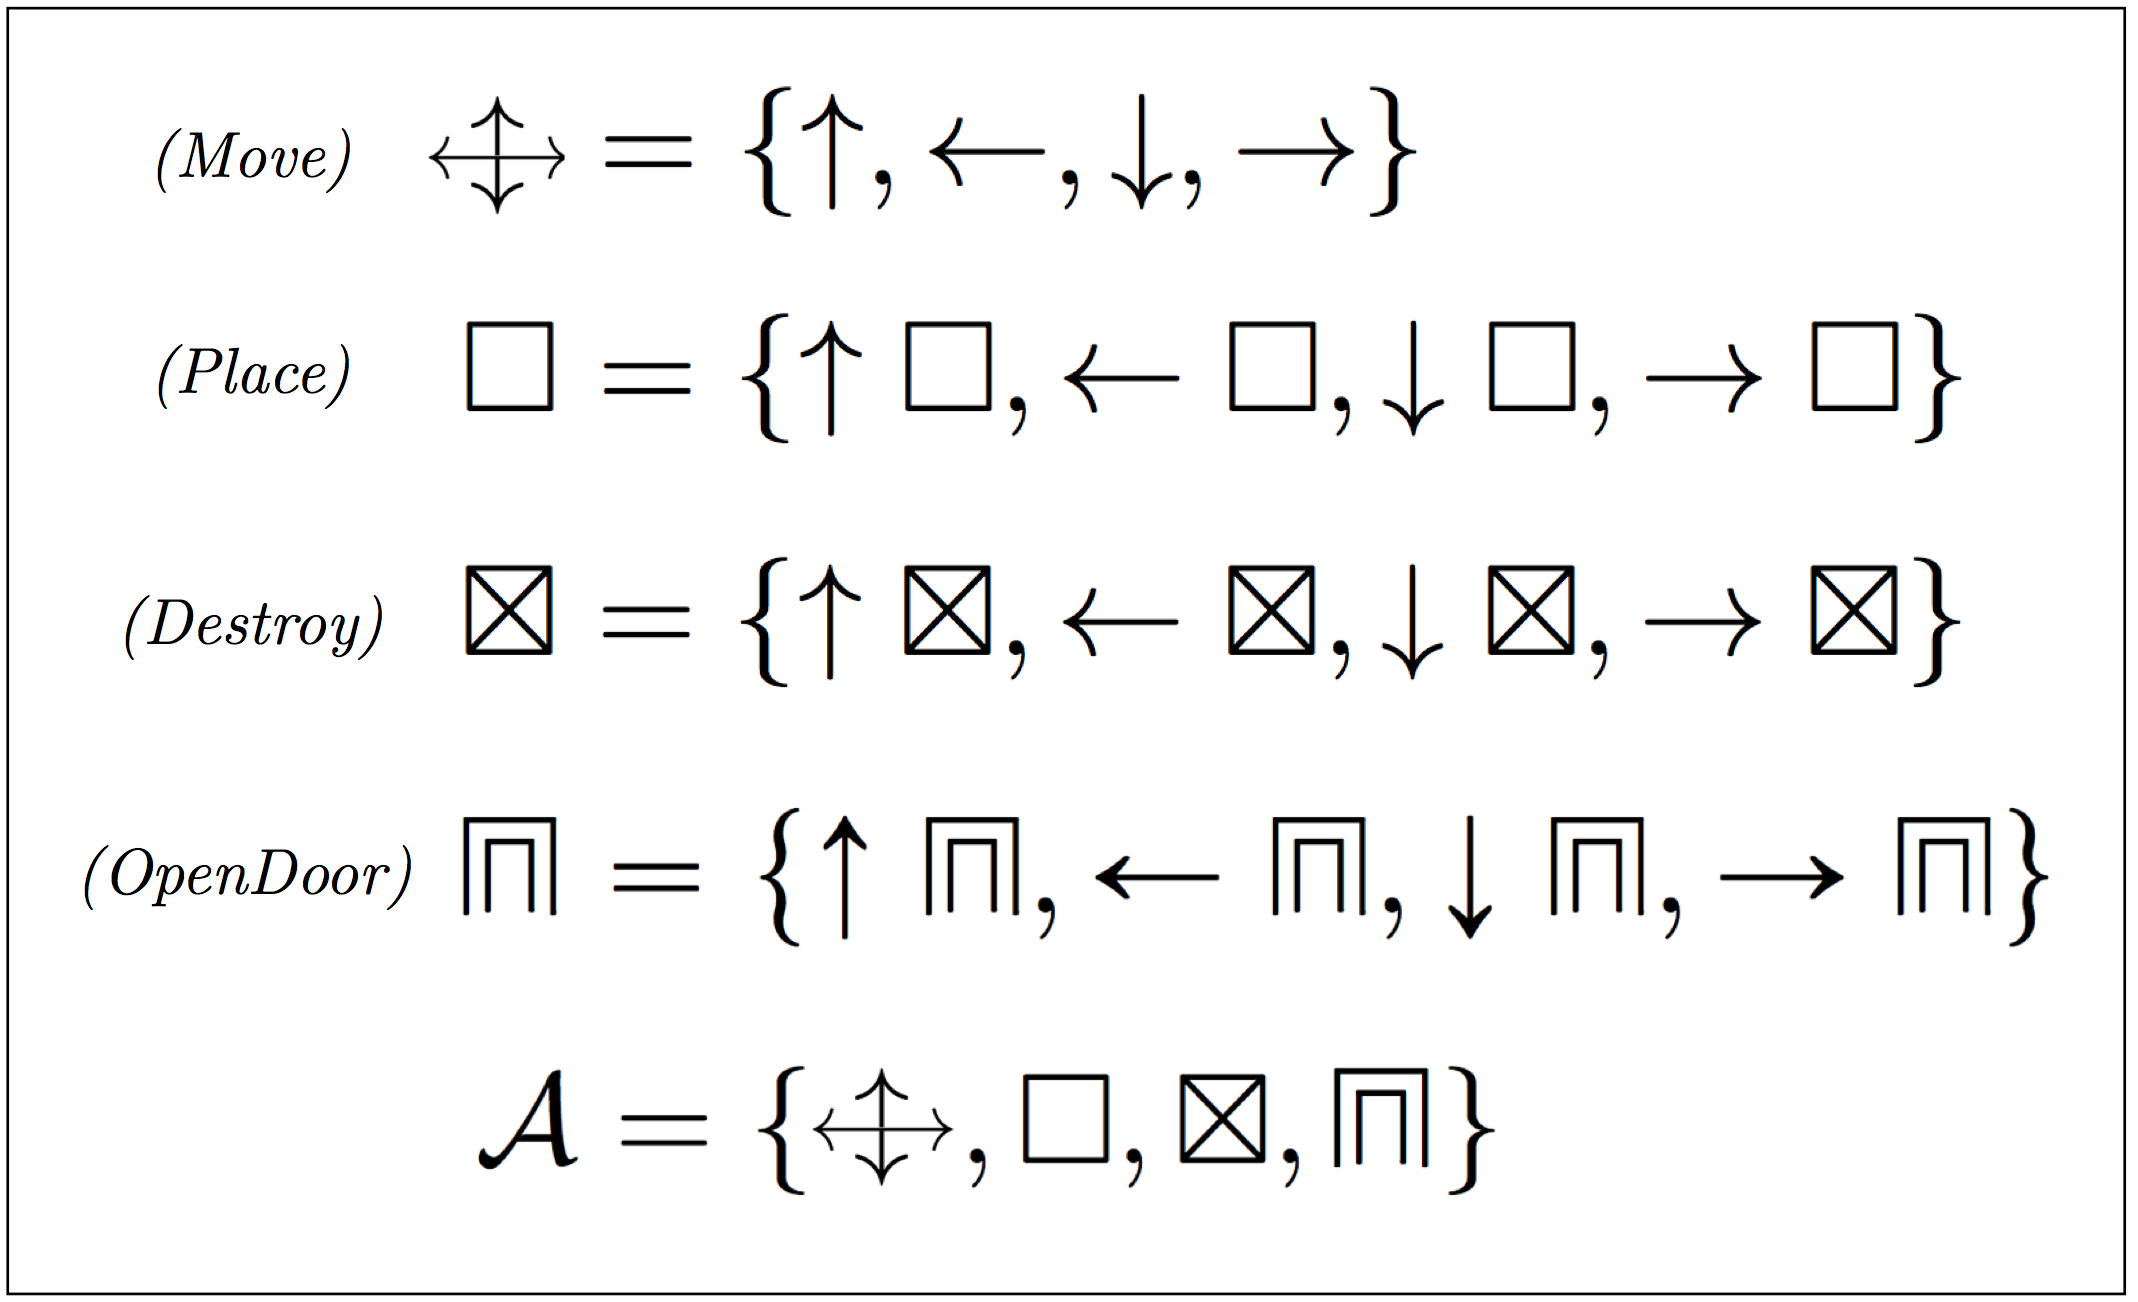
\includegraphics[scale = 0.15]{figures/all_actions.png}
%\caption{The set of all actions in the Minecraft domain. \label{fig:all_actions} \dnote{We could consider simplifying this figure to only include the action symbol (e.g. $\square$) and get rid of the arrows to indicate that it is a `directioned' action}}
%\stnote{Agree about removing directional arrows.  Actually, I thought there was a version of this figure with ``bridgeworld'' vs ``vi''a ction space that was effective.  Just showing the legend graphically as this version does doesn't add much.  So I'd say, cut this figure, or add back the ``vi'' vs ``affordance'' plannign version of the figure.  }
%\end{figure}

While the OO-MDP state definition is a good fit for the Minecraft
domain, our motivation for using an OO-MDP lies in the ability to
formulate predicates over classes of objects. That is, the OO-MDP
definition also includes a set of predicates ${\cal P}$ that operate
on the state of objects to provide additional high-level information
about the MDP state. For example, in \texttt{BRIDGEWORLD}, a ${\tt
  nearTrench}({\tt AGENT})$ predicate evaluates to true when the singular
instance of class $\texttt{ AGENT}$ is directly adjacent to an empty location
at floor level (i.e. the cell beneath the agent in some direction does not
contain a block). In the original OO-MDP work, these predicates were used
to model and learn an MDP's transition dynamics. In the next section,
we use the predicates to define affordances that enable planning
algorithms to prune irrelevant actions.


% As we will
%see in section 3, this helps us form preconditions and goals that
%generalize beyond a particular instance of a state space.

%As with a classical finite MDP, planning with an OO-MDP involves
%running value iteration to determine a policy.  Reward propagation in
%value iteration occurs as in a Bellman update:
%\begin{align}
%U_{i+1}(s) \leftarrow \mathcal{R}(s) + \gamma \max_{a \in \mathcal{A}(s)} \sum_{s'} \text{Pr}(s' \mid s, a)U_i(s')
%\end{align}
%Where $U_i(s)$ is the {\it utility} of state $s$ at iteration $i$, 
%representing the expected reward of being in that state. See Algorithm \ref{alg:vi} for the full pseudocode of the algorithm ~\citep{russellnorvigAI}.%

%% VI pseudocode from Norvig/Russell
%\begin{algorithm}
%  \caption{Value-Iteration($\mathcal{A}$, $\mathcal{R}$, $\mathcal{S}$, $\epsilon$, $\gamma$) \\ {\it Complexity:} $\mathcal{O}(|\mathcal{A}|\cdot |\mathcal{S}|^2)$}
%  \begin{algorithmic}[1]
%    \While {$\delta < \epsilon \frac{(1-\gamma)}{\gamma}$}
%    \State $U \gets U';\delta \gets 0$
%    \For {each state $s \in \mathcal{S}$}
%    \State $U'[s] \leftarrow \mathcal{R}(s) + \gamma \max_{a \in \mathcal{A}(s)} \sum_{s'} \text{Pr}(s'\mid s,a) U[s']$
%    \If {$|U'[s] - U[s]| > \delta$}
%    	\State $\delta \gets |U'[s] - U[s]|$ 
%    \EndIf
%    \EndFor
%    \EndWhile \\
%    \Return U;
%  \end{algorithmic}
%  \label{alg:vi}
%\end{algorithm}%
%

%In practice, Value Iteration scales very poorly, either as the state
%space grows, or the action set grows. This is because the state-action
%space, depending on the domain, grows exponentially in the number of
%actions.  This problem is ameliorated slightly by introducing the
%OO-MDP, but it still fails in just about all of the planning scenarios
%we introduce here because the agent explores all states that result
%from applying every action in every state.  The complexity of Value-Iteration
%is known to be $\mathcal{O}(|\mathcal{A}||\mathcal{S}|^2)$, so as the number
%of states increases, the runtime of Value Iteration grows quite quickly.



\section{AFFORDANCES}
\label{sec:affordances}

%% Formalism
In many planning scenarios, not all actions are needed in all
states. In fact, many applications of actions in states do not
contribute toward solving the planning task, but instead, cause the
state-space to grow exponentially. This is especially true in domains in which
the agent's actions can drastically shape the environment, such as in
Minecraft. As discussed above, the affordances that an 
agent perceives are determined by the agent's current goal. We define an affordance $\Delta$, 
as a tuple, $\langle p,g\rangle\ \longmapsto \alpha$,
where:
\begin{itemize}
\item[] $\alpha$ a subset of the action space, $\mathcal{A}$, representing the relevant {\it action-possibilities} of the environment.
\item[] $p$ is a predicate on states, $s \longrightarrow \{$0$, 1\}$
  representing the {\em precondition} for the affordance.
\item[] $g$ is a lifted goal description, represented as an ungrounded predicate on states, $g$.
\end{itemize}

The precondition, $p$ refers to a predicate over an OO-MDP state,
where an OO-MDP state is represented as a union of all of the objects'
current attribute values: $\cup_{i = 1}^o o_i.state$.  The use of an
OO-MDP here makes predicates more general tasks (e.g. OO-MDP
predicates may be relational) and is one of the reasons that
affordance-aware planners may be untethered from specific state
spaces, as the predicate of $p$ benefit from the richness of the
predicates of an OO-MDP. Further, the lifted goal description, $g$, is
an ungrounded predicate, describing the type of task being solved. In
Minecraft, this can range from reaching a particular coordinate
($reachGoal$), to constructing an object of a certain type
(e.g. smelting gold, building a pickaxe). $p$ is intended to parallel
the agent's most salient observations of its environment, and $g$
represents the type of task the agent is currently trying to achieve -
this results in a small set of action-possibilities $\alpha$, that
help the agent achieve its goal.

\begin{algorithm}
  \caption{pruneActions($state$, {\it KB}) \\ {\it Complexity:} $\mathcal{O}(|\text{{\it KB}}|)$}
  \begin{algorithmic}[1]
    \For {$\Delta \in $ {\it KB}}
    \If {$\Delta.p(state)$ and $\Delta.g == state.goal$}
    \State $\alpha.update(\Delta.p, \Delta.g)$
    \EndIf
    \EndFor \\
    \Return $\alpha$
  \end{algorithmic}
  \label{alg:prune_actions}
\end{algorithm}


The pseudocode for how an affordance-aware agent prunes its actions
may be seen in Algorithm \ref{alg:prune_actions}. For instance, if the
agent is at the trench in \texttt{BRIDGEWORLD} and is faced with a
$reachGoal$ task, then the agent would not consider placing a block in
any arbitrary location, as that would not further its ability to reach
the goal. Instead, we provide\footnote{Currently, we provide a
  planning agent with annotated affordances. However, our next step is
  to pursue learning affordances directly} the agent with the
following affordance: $\Delta_1 = \langle nearTrench, reachGoal
\rangle \rangle \longmapsto \{\square\}$, that tells the agent to try
placing blocks when next to a trench (as the trench could inhibit its
progress toward reaching the goal). So, in any $reachGoal$, the
action-possibilities of placing a block are only included in $\alpha$
when the predicate $nearTrench$ is true for the agent. For most
$reachGoal$ tasks, we also provide the following affordances:
$\Delta_2 = \langle onPlane, reachGoal \rangle \rangle \longmapsto
\{\updownarrow \leftrightarrow\}, \\ \Delta_3 = \langle nearWall,
reachGoal \rangle \longmapsto \{\boxtimes \}$.  These two eliminate
the possibility of applying the ``destroy" action in every state.  As
a result, the planner avoids exploring every consequent state in which
that block has been destroyed, enabling an affordance-aware planner in
$reachGoal$ task types to handle large state spaces.

%% Further, agents may be equipped with affordances with differing lifted
%% goal descriptions, thus enabling an agent with a single, relatively
%% minimal knowledge base to tackle planning problems of scale from a
%% variety of goal types.

We propose the notion of an {\it affordance-aware} planner, which
refers to a planning algorithm that prunes the actions set according
to a knowledge base of affordances. Pruning the action set affects
different planning algorithms in different ways. In particular, we
focus on how action pruning benefits {\em dynamic programming}, {\em
  policy rollout}, and {\em subgoal} planning paradigms in the
following sections.

\subsection{Dynamic Programming}
In dynamic programming paradigms, the planning algorithm estimates the
optimal {\em value function} for each state. Formally, the optimal
value function ($V^*$) defines the expected discounted return from
following the optimal policy in each state:
\begin{equation}
\label{eq:bellman}
V^*(s) = \max_{a \in \mathcal{A}(s)} \sum_{s'} \text{Pr}(s' \mid s, a)\left[\mathcal{R}(s,a,s') + \gamma V^*(s') \right];
\end{equation}
this equation is known as the Bellman
equation~\citep{bellman57}. Given the optimal value function, the
optimal policy is derived by taking the action that maximizes the
values of each state; that is, by taking the action with the
highest optimal state-action value:
\begin{equation}
\label{eq:qvalue}
Q^*(s,a) = \sum_{s'} \text{Pr}(s' \mid s, a)\left[\mathcal{R}(s,a,s') + \gamma V^*(s') \right].
\end{equation}
Dynamic programming planning algorithms (such as Value
Iteration~\citep{bellman57}) estimate the optimal value function by
initializing the value of each state arbitrarily and iteratively
updating the value of each state by setting its value to the result of
the right-hand-side of the Bellman equation using its current estimate
of $V$ instead of $V^*$. Iteratively updating the value function
estimate in this way is guaranteed to converge to the optimal value
function.

Using a pruned action set in dynamic programming can accelerate its
computation in two ways: (1) by reducing the number of actions over
which the max operator in the Bellman equation must iterate and (2) by
restricting the state space for which the value function is estimated
to the states that are reachable with the pruned action set from the
initial state. Note that neither of these computational gains come at
the cost of solution optimality as long as the pruned action set
contains the actions necessary for an optimal policy from the initial
state. In the case of the Bellman equation, the max operator makes the
value function indifferent to the effects of actions that are not part
of the optimal policy; therefore, the action set can be reduced
entirely to the actions in the optimal policy without sacrificing
optimality. Similarly, since we are only concerned with finding a good
policy to dictate behavior from some initial state, the state space
for which the value function is computed can be reduced to that which
is reachable using only the optimal actions without sacrificing
optimality.  
%\stnote{So the stuff about not sacrificing the optimal
%  policy seems right, but I wonder if we can say something more formal
%  about what has to be true about affordances in order for affordance
%  planning to still be optimal.}
%\dnote{Agreed - that would be a compelling bit to include, though I think
%we're ironing out the details of affordances still (more to come in our next email). So
%for now I vote we table this until a few days down the line}

\subsection{Policy Rollout}

In policy rollout planning paradigms, the agent starts with some
initial policy and follows it (or rolls out the policy) from an
initial/current state to either some maximum time horizon or until a
terminal state is reached. Often, these approaches use samples from
the policy rollout to improve estimates of the value function and
indirectly improve the rollout policy. Examples of planning algorithms
in this paradigm include Monte Carlo methods~\citep{browne12,
  silver10} and temporal difference
methods~\citep{sutton99,sutton1988lpm,rummery1994line,6313077,lagoudakis2003least,Peters:2008ve}.
By using a pruned
action set, the policy space, and resulting state space explored from
the searched policies, is reduced, thereby reducing the number of
rollouts necessary to find a good policy. Similar to dynamic
programming paradigms, as long as the pruned action set contains
actions necessary for the optimal policy, solution optimality will not
be sacrificed.

In this work, we will explore how real time dynamic programming
(RTDP)~\citep{barto95} benefits from affordances. RTDP is both a
dynamic programming algorithm and a policy rollout algorithm. RTDP
starts by initializing the value function optimistically. It then
follows a greedy rollout policy with respect to its currently
estimated value function. After each action selection in the policy
rollout, RTDP updates its estimate of the value function for the last
state using the Bellman equation. RTDP is guaranteed to converge to
the optimal policy from some initial state and has the advantage that
it iteratively refocuses its attention to states that are likely to be
on the path of the optimal policy.  \stnote{Need a sentence about why
  RTDP vs other methods reviewed above.}

In affordance-aware RTDP, the action selection of the rollout policy
is restricted to the affordance-pruned action set and the Bellman
equation is similarly restricted to operating on the affordance-pruned
action set.



%The Affordance Value-Iteration algorithm (for full pseudocode see Algorithm \ref{alg:aff_vi}) works by
%only enumerating a subset of the actual state space. More specifically, the state space is generated
%outward from the agent's start state by applying actions that are deemed relevant by the current
%set of affordances. Thus, in most cases, a much smaller state space $\hat{\mathcal{S}}$ is produced,
%on which Value-Iteration finds an optimal policy.%
%
%

%\begin{figure}
%\centering
%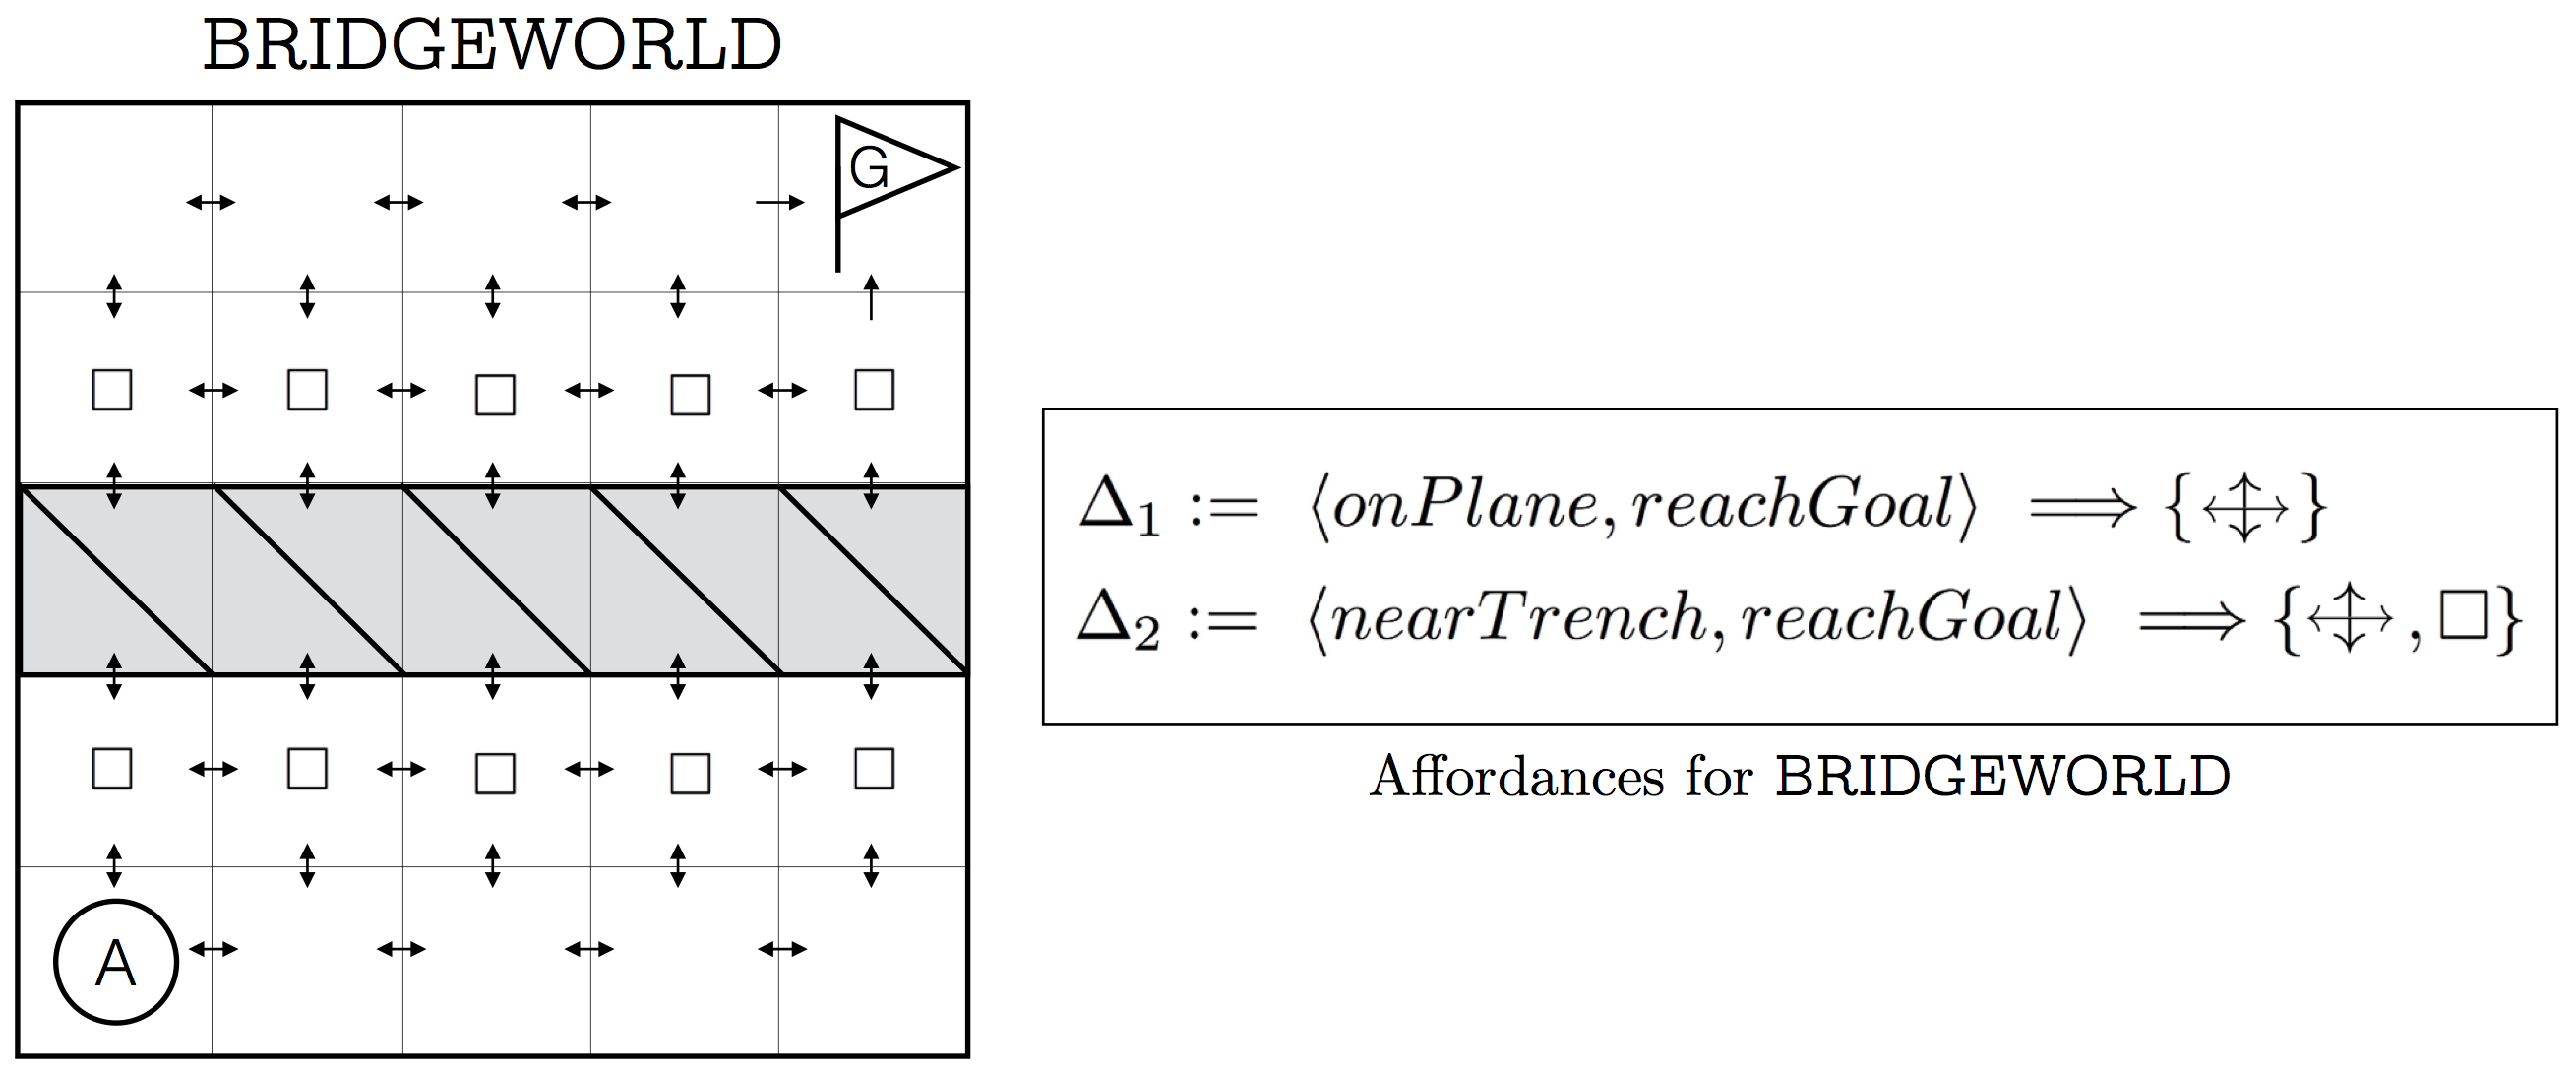
\includegraphics[scale=0.22]{figures/bridgeworld_aff.png}
%\caption{The affordance planner's state-action space on \texttt{BRIDGEWORLD}.}
%\label{fig:bridgeworld_aff}
%\end{figure}%

%Furthermore, given perfect subgoal knowledge for a
%particular planning task, the affordance formalism will find an
%optimal policy {\it extremely} quickly. We imagine extensions in which
%an agent gets stuck and must ask a human partner for help using
%natural language, and the resulting dialog could endow the agent
%with subgoal knowledge. This also allows the agent to prune way
%unnecessary actions in $\mathcal{A}$ in each specific planning task,
%making it possible to solve a engage with a large number of planning
%scenarios that may call for different actions. %
%

%% VI pseudocode + Affordances
%\begin{algorithm}
%  \caption{Affordance-VI($\mathcal{A}$, $\mathcal{R}$, $s_0$, $kb$, $goal$, $\epsilon$, $\gamma$) \\ {\it Complexity:} $\mathcal{O}(|\mathcal{A}|\cdot |\hat{\mathcal{S}}|^2)$}
%  \begin{algorithmic}[1]
%    \State $\hat{\mathcal{A}} \gets pruneActions(kb, s_0, \mathcal{A}, goal)$
%    \State $\hat{\mathcal{S}} \gets genStates(kb, \hat{\mathcal{A}})$
%    \While {$\delta < \epsilon \frac{(1-\gamma)}{\gamma}$}
%    \State $U \gets U';\delta \gets 0$
%    \For {each state $s \in \hat{\mathcal{S}}$}
%    \State $U'[s] \gets \mathcal{R}(s) + \gamma \max_{a \in \hat{\mathcal{A}}(s)} \sum_{s'} \text{Pr}(s'\mid s,a) U[s']$
%    \If {$|U'[s] - U[s]| > \delta$}
%    	\State $\delta \gets |U'[s] - U[s]|$ 
%    \EndIf
%    \EndFor
%    \EndWhile\\
%    \Return U;
%  \end{algorithmic}
%  \label{alg:aff_vi}
%\end{algorithm}%

%In the worst case, the Affordance-Value-Iteration Algorithm is 
%bounded by $\mathcal{O}(|\mathcal{A}|\cdot |\hat{\mathcal{S}}|^2)$, where
%$\hat{\mathcal{S}}$ is the subset of the states that were reachable using the
%resulting pruned action set determined by the agent's affordances. Thus,
%if the affordances were poorly designed, then the lower bound for the size of
%$\hat{\mathcal{S}}$, is precisely the full state space, $\mathcal{S}$. However,
%in general, when reasonable affordances are applied the agent is guaranteed to prune its
%action set for any number of states, and thus will explore less of the state space
%as a result.%

%The affordance formalism introduced above and expanded on in this
%paper resolves the weaknesses of these other frameworks by limiting
%the complexity of the seed knowledge required of the designer, while
%still providing enough knowledge to limit the search space but also
%maintain scalability.



\subsection{Subgoal Planning}
\label{sec:subgoals}

Subgoal planning leverages the intuition that certain goals in
planning domains may only be brought about if certain preconditions
are first satisfied. For instance, in the bridge problem, the agent must
first place a block in the trench to create a bridge before crossing
the trench.  \citet{branavan12a} explore learning subgoals from the
Minecraft wiki and applying them in order to plan through a variety of
problems in Minecraft.

% Formalism
Formally, in subgoal planning, the agent is given a set of subgoals, where each subgoal is a pair of predicates:
\begin{align}
SG = \langle x_k, x_l \rangle
\end{align}

where $x_l$ is the effect of some action sequence performed on 
a state in which $x_k$ is true. Thus, subgoal planning requires 
that we perform high-level planning in subgoal space, and low-level 
planning to get from subgoal to subgoal. The low-level planner may vary, though
Metro-FF and A* are popular choices (depending on domain constraints), as is Value Iteration.

In the case of \texttt{BRIDGEWORLD}, the agent might consider placing
a block somewhere along the trench to be a subgoal. Then, it runs
a low-level planner to get from its starting location to the subgoal.
Next, it runs the same low-level planner from the first subgoal to the finish.
Subgoals enhance an agent's planning abilities when they propose {\it
  necessary} claims about the domain. If the subgoals are {\it
  contingent} (i.e. true in some state spaces of the domain but not in
others), then they do not limit the search space (and in fact can negatively 
effect planning). For instance, consider the task in \texttt{BRIDGEWORLD}, 
in which the agent must place a block in the trench that separates the agent 
from the goal. The subgoal $\langle blockInTrench, reachGoal\rangle$ might be a
perfectly useful subgoal in \texttt{BRIDGEWORLD}, but an adversary
could easily come up with thousands of worlds in which such a subgoal
would completely derail the agent's planner. Thus, many subgoals do
not scale beyond a particular instance of a state space. In order for
subgoals to be useful, they must be necessary claims about the domain,
otherwise, one can always come up with a counter world (by definition
of necessary).  Compare this scenario to the problem of baking bread
in Minecraft: possessing grain is always required to make bread, and it
is impossible to construct a world where this precondition is not
true.

Subgoal planners benefit in many ways by being made affordance-aware.
One of the main problems of subgoal planning is that subgoal planners
re-explore large portions of the state space, as illustrated by
Fig. \ref{fig:bwsg}. The affordance-aware version of subgoal planners
will tend to avoid this problem by focusing on actions that are likely
to direct the agent to the goal. Since subgoals are handcrafted to be
preconditions for arriving at the goal, a large portion of the state
space should will be pruned away (namely, the portion that is only
accessible through actions that do not take you toward the goal).
Furthermore, the low-level planners still suffer from all of the
standard issues of planning we have discussed above; particularly in
the Minecraft domain, planners cannot scale to accommodate that state
space sizes that are possible in Minecraft (and thus, the real
world). Thus, we may make subgoal planners affordance-aware by
equipping the subsequent low-level planners with affordances in order
to plan efficiently from subgoal to subgoal. What makes affordances
especially useful to subgoal planning, is that as long as the subgoals
are defined using OO-MDP predicates, each subgoal may activate a
different set of affordances, thereby even more greatly focusing the
search.


%{\bf Problem 2: Efficient Search} The last problem with subgoal
%planning is that the use of subgoals actually requires that we
%research a huge portion of the state space. Consider the
%\texttt{BRIDGEWORLD} example in which the subgoal is to place a block
%along the trench somewhere - once we plan from the state in which a
%block has been placed at the trench, Value Iteration will search paths
%exploring both sides of the trench rather than focusing on the
%opposite side of the trench toward the goal.


%A final, but less significant problem, is that Subgoal planning still 
%requires the use of Value Iteration or another low-level planner, which does not scale well - if 
%there is ever a case in which planning between two subgoals is 
%at all complex, then Subgoal planning is out of luck.


\section{EXPERIMENTS}

%\jmnote{Reminder that this should be updated to be with respect to
%  RTDP as a baseline and ideally should include a performance metric
%  specifying the number of state backups that were used.}
%
%\stnote{Experiments and results should be merged.  Also I think we
%  need to think through how to structure the results. }

%\stnote{To write the experiments section, it's good to say what we are
%  interested in learning first.  What are we testing?  What is our
%  hypothesis?  Then explain the setup, then explain what the results
%  say about the hypothesis.  I would make experiments and results one
%  section, with subsections for each experiment + results}

We conducted a series of experiments in the Minecraft domain that
tested standard planners from each planning paradigm: Value Iteration,
RTDP, and Subgoal planning (with RTDP as the low-level planner). These
planners were compared with {\it affordance-aware} versions of each
algorithm tasked with the same set of problems. We selected the
affordances provided from our background knowledge of the domain. The
agent was given a knowledge base 15 affordances. Our experiments consisted of a
variety of tasks, ranging from basic path planning, to baking bread,
to opening doors and jumping over trenches.  We also tested each
planner on worlds of varying size and difficulty to demonstrate the
scalability and flexibility of the affordance formalism. The
evaluation metric for each trial is the number of state backups that
were executed in each iteration of each planning algorithm. Value
Iteration was terminated when the maximum change in the value function
was less than 0.01. RTDP terminated when the maximum change in the
value function was less than 0.01 for ten consecutive policy
rollouts. In subgoal planning, the high-level subgoal plan was solved
using breadth-first search; which only took a small fraction of the
time compared to the total low-level planning and therefore is not
reported.

The reward function was defined as uniformly $-1$ except for states in
which the agent stood in lava, which were given $-200$ reward (lava
states were non-terminal). The goal was set to be terminal, and also
initialized with a reward of $-1$. This was done in order to allow for
an optimistic RTDP value initialization\footnote{Note that since the
  goal is terminal, it will still be better than any other state, as
  it is a means of ceasing to accrue negative reward}. The discount
factor was set to $\lambda = 0.99$ with a minimum $\delta$ required
for concergance of $0.01$.


Our entire set of experiments were run using stochastic actions. For all actions that were associated with a direction (e.g. movement, block placement, jumping), with low probability ($0.1$) the executed action has the unintended effect of being applied in the reverse direction.

\subsection{RESULTS}


% === NOTE: OLD RESULTS ==== (time)
%\begin{table}
%\begin{tabular}{ l || c | c | c }
%  & Affordances & Subgoals & VI \\
%  \hline
%  \texttt{10WORLD} 		&	{\bf 0.6s} 		&	 1.8s 		& 1.1s  \\
%  \texttt{13WORLD} 		&	{\bf 2.5s} 	 	& 	10.1s 		& 6.0s  \\
%  \texttt{15WORLD} 		&	{\bf 6.7s} 	 	& 	21.6s 		& 11.8s  \\
%  \texttt{17WORLD} 		& 	{\bf 16.6s} 	& 	45.4s 		& 28.2s  \\
%  \texttt{20WORLD} 		& 	{\bf 57.6s} 	& 	144.3s 		& 140.5s  \\
%  \texttt{JUMPWORLD}  	& 	{\bf 4.3s} 		& 	21.1s 		& 10.1s \\
%  \texttt{BREADWORLD}  	& 	25.5s		& 	{\bf 22.8s} 	& 51.6s \\
%  \texttt{DOORWORLD}  	& 	{\bf 16.3s} 	& 	25.0s 		& 25.3s \\
%  \texttt{MAZEWORLD}  	& 	{\bf 17.9s} 	& 	114.8s		& 37.6s \\
%  \texttt{HARDWORLD} 	& 	{\bf 34.5s}  	& 	215.9s 		& 149.7s
%\end{tabular} 
%\label{results_1}
%\caption{Tests on a variety of tasks without block placement and destruction actions}
%\end{table}
%
%\vspace{4 mm}
%
%\begin{table}
%\begin{tabular}{ l || c | c | c }
%  & Affordances & Subgoals & VI \\
%  \hline
%  $|\mathcal{A}| = 4$ 		& 	6.7s 	& 	11.8s 	& 6.7s  \\ % Just movement
%  $|\mathcal{A}| = 8$ 		& 	6.8s 	& 	25.4s 	& 14.8s  \\ % + openDoor
%  $|\mathcal{A}| = 12$ 	& 	6.8s 	& 	39.8s 	& 22.9s  \\ % + Oven
%  $|\mathcal{A}| = 13$ 	& 	6.8s 	& 	41.28s      & 24.7s  \\ % + grain
%  $|\mathcal{A}| = 17$ 	& 	6.7s	& 	55.5s	& 33.1s  \\ % + 0 blocks, placement
%  $|\mathcal{A}| = 17$ 	& 	6.8s 	& 	DNF 		& DNF  \\ % + 1 blocks, placement
%  $|\mathcal{A}| = 21$ 	& 	6.6s 	& 	DNF 		& DNF  \\ % + destruction
%\end{tabular}
%\label{results_2}
%\caption{Plan on the simplest possible task (path planning in a flat plane with no obstacles - \texttt{15WORLD}) with incrementally larger action sets.}
%\end{table}
%


% ==== DETERMINISTIC RESULTS =====
\begin{table}
\scalebox{0.75}{
\begin{tabular}{ l || c | c | c | c | c | c }
  & VI & RTDP & SG & A-VI & A-RTDP & A-SG \\
  \hline
  \texttt{4BRIDGE} 		&	39015 		& 2368 		&		3674 	& 9660  		& 259 	& 214  \\
  \texttt{6BRIDGE} 		&	162945 	 	& 4894 		&		4403  	& 23000  		& 916 	& 473  \\
  \texttt{8BRIDGE} 		&	496179 	 	& 16873 		&		? 		& 41860		& 1975 	& 944  \\
%  \texttt{10BRIDGE} 		&	1565190^ 	 	& 54115^ 		&		?	 	& 66240	 	& 3889	  	& 1399	\\
  \texttt{DOORB} 		&	312579 	 	& 11782 		&		11322	& 92460	 	& 3285  	& 1482	\\
  \texttt{LAVAB}  		&	177174 	 	& 3242 		&		4490		& 41860	 	& 717  	& 359\\
  \texttt{TUNNEL}  		&	196810 	 	& 30676		&		6443 	& 51430	 	& 581  	& 220	\\
  \texttt{BREAD}  		&	26502 	 	& 8501 		&		8564 	& 1554	 	& 1124  	& 589
\end{tabular}
}

\caption{The number of state backups performed by each algorithm for a
  variety of tasks requiring block placement and destruction.
  Affordances dramatically improve performance.  \dnote{Ongoing
    experiments.}\label{table:blocks} \stnote{Bold best performing entry.}}
\end{table}

\begin{table}
\scalebox{0.75}{
\centering
\begin{tabular}{ l || c | c | c | c | c | c}
  & VI & RTDP & SG & A-VI & A-RTDP & A-SG \\
  \hline
  \texttt{10WORLD} 		&	1600		& 1369 	&	1166		&	1600	 	& 	1408 	&	1051	\\
  \texttt{15WORLD} 		&	5850		& 5920 	&	4168 	&	5850	 	& 	4042 	&	6016 	\\
  \texttt{20WORLD} 		&	14400	& 15645 	&	18400.	&	14400	& 	16233 	&	15345	\\
  \texttt{JUMP}  			&	2940		& 2857 	&	2323 	&	2940	 	& 	2435 	&	2146	\\
  \texttt{DOOR}  		&	6315		& 2952 	&	3122 	&	6315	 	& 	3075 	&	2104 	\\
  \texttt{MAZE}  			&	4266		& 2857 	&	1961 	&	4266	 	& 	2665 	&	1418	\\
  \texttt{LAVA} 			&	800		& 698	&	570 		&	800	 	& 	638 		&	494	\\
  \texttt{HARD} 			&	16588	& 7359 	&	3295 	&	16588 	& 	6611 	&	3413\\
\end{tabular} 
}

% ==== NON-DETERMINISTIC RESULTS =====
\begin{table}
\scalebox{0.75}{
\begin{tabular}{ l || c | c | c | c | c | c }
  & VI & RTDP & SG & A-VI & A-RTDP & A-SG \\
  \hline
  \texttt{4BRIDGE} 		&	71604 		& 836 		&		1373 	& 100  		& 152 	& 141  \\
  \texttt{6BRIDGE} 		&	413559 	 	& 4561 		&		28185  	& 366  		& 392 	& 547  \\
  \texttt{8BRIDGE} 		&	496179 	 	& 16873 		&		28185 		& 366		& 392 	& 547  \\
  \texttt{DOORB} 		&	312579 	 	& 11782 		&		11322	& 92460	 	& 3285  	& 1482	\\
  \texttt{LAVAB}  		&	177174 	 	& 3242 		&		4490		& 41860	 	& 717  	& 359\\
  \texttt{TUNNEL}  		&	196810 	 	& 30676		&		6443 	& 51430	 	& 581  	& 220	\\
  \texttt{BREAD}  		&	26502 	 	& 8501 		&		8564 	& 1554	 	& 1124  	& 589
\end{tabular}
}

\caption{The number of state backups performed by each algorithm for a
  variety of tasks requiring block placement and destruction.
  Affordances dramatically improve performance.  \dnote{Ongoing
    experiments.}\label{table:blocks} \stnote{Bold best performing entry.}}
\end{table}

\begin{table}
\scalebox{0.75}{
\centering
\begin{tabular}{ l || c | c | c | c | c | c}
  & VI & RTDP & SG & A-VI & A-RTDP & A-SG \\
  \hline
  \texttt{10WORLD} 		&	800		& 1205 	&	1263		&	800	 	& 	985 	&	960	\\
  \texttt{15WORLD} 		&	3150		& 3939 	&	3328 	&	3150	 	& 	3089 	&	2331 	\\
  \texttt{20WORLD} 		&	7200		& 10719 	&	8738		&	7200		& 	8004 	&	6099	\\
  \texttt{DOOR}  		&	6315		& 5646 	&	4104 	&	6315	 	& 	4059 	&	2886	\\
  \texttt{JUMP}	  		&	2940		& 4313 	&	4262 	&	2940	 	& 	3548 	&	2922 	\\
  \texttt{MAZE}  			&	4266		& 5648	&
  \texttt{LAVA} 			&	800		& 1328	&	1003 	&	800	 	& 	861 		&	772	\\
  \texttt{HARD} 			
\end{tabular} 
}

\caption{The number of state backups performed by each algorithm for a
  variety of tasks without block placement and destruction actions.
  Here affordances have a minimal effect. \dnote{Ongoing
    experiments.}\label{table:noblocks}}

\end{table}


% === NON-DETERMINISTIC RESULTS ===
% we have them, still need to put into tables (which will be done tonight 3/10/14)

%
%As one can see from Table \ref{results_2}, in those cases where
%$|\mathcal{A}| = 21$ and $|\mathcal{A}| = 25$, the only planning algorithm to
%actually complete the tasks was the affordance planner. This is because each
%of these cases scaled to include block destruction and block placement actions.
%Thus, any case in which these actions are required to complete the task at hand,
%only affordance planning will succeed. This is significant, as Table \ref{results_1}
%indicates that the affordance planner plans more effectively than the other
%systems, but it can also handle novel problems involving those actions that
%alter the environment in sever ways.
%
%We also include a Bonus round indicating
%those tasks that only the affordance planner was able to solve. Finally, since
%each affordance is attached to a particular goal, a single knowledge base will
%scale across state-spaces and task types, causing affordance planning to be
%extremely transferable. Additionally, we plan to add experiments in
%Non-deterministic planning scenarios, as well as testing on the planning scenarios
%from table \ref{results_1} where the knowledge bases remain constant across
%state-spaces to test the generality of each algorithm.

%% In all experiments, the agent
%% was given a non-deterministic action set.  All of the bridge worlds
%% had a trench prohibiting the agent from reaching the goal. In order to
%% solve one of these tasks, the agent needed to build a bridge over (by
%% placing a block). We also tested on worlds that included lava, doors
%% the agent had to open, a world that required the agent find some grain
%% and bake bread, and a world where a wall stood between the agent and
%% the goal and the agent needed to cut down the wall to reach the
%% goal. For testing, we used RTDP as the low level planner for the
%% Subgoal Planner as well as for the affordance aware Subgoal Planner.

Table~\ref{table:blocks} shows the results of running the standard
planners and their affordance aware counterparts on a set of tasks
that require the use of block placement and/or destruction.  The
affordance aware planners significantly outperformed their unaugmented
counterparts in the majority of these experiments. They proved
especially effective when paired with subgoals, as can be seen by the
results of the affordance aware subgoal planner, demonstrating that
affordances are particularly useful if subgoal knowledge is known.
Subgoals combined with affordances allow different types of pruning to
occur depending on what the agent is trying to accomplish at each
stage. In other words, when the agent is trying to find grain, it will
focus on grain finding actions; when it is trying to bake bread, it
focuses on bread baking actions.  Additionally, affordance aware VI
and affordance aware RTDP outperform their unaugmented versions.  This
result demonstrates that affordances prune away many useless action in
these block building, block destruction, and bread baking types of
tasks.

Table~\ref{table:noblocks} shows the results of running the standard
planners and their affordance-aware counterparts on tasks that do {\it
  not} require the use of block placement and destruction.  In these
cases, the affordance awareness did not improve any of the planners
from their baseline versions. Affordances are only beneficial when
they allow an agent to prune actions which could combinatorially alter
the state space. In each of these worlds, the agent only needed to
move itself through the environment, rather than alter the
environment.  

\dnote{Part of me thinks that we should come up with a term for these
  action types (e.g. ``harsh" actions) that have this combinatoric
  effect on the state space size. This might help in clarifying when
  an affordance aware planner is helpful (currently we split our
  results into two action types, which might be good enough.  }
\stnote{I'm okay with a term for these types of actions, but I just
  edited it out for now because we need to formally define it earlier
  and use it consistently throughout the paper.  We shoudl maybe talk
  about it first.}


These results highlight where affordances highlights the fact that affordance aware planers are
not always the right way to fix planning scalability issues - while
effective in many cases, they do not always benefit planners. For one,
they are specific to task types, as the lifted goal description $g$ of
each affordance must be defined with a task type (e.g. a predicate
that defines the goal) in mind. Additionally, affordances (if defined
optimally) only prune away actions that are useless in achieving the
goal, but fail to prune away actions whose importance is not easily
inferred. For instance, in \texttt{BRIDGEWORLD}, when the agent is up
against a trench, it will still explore the space in which it places
blocks behind it, and to its side, despite the fact that these are not
useful applications of the place action. In future work, we would like
to change the precondition $p$ to a set of features that represent the
salient portions of the agent's current state and output a
distribution over the agent's action set. This would allow an
affordance aware planner to {\it prioritize} and rank actions in each
state, which would lead to pruning much larger portions of the
state-space.


The final factor to consider when augmenting a planner with affordances is whether or not the desired domain provides
the agent with actions that can dramatically affect the state space. If the action set is relatively small and the actions
don't significantly impact the shape of the state-space with each application, then affordances are not likely to help. For instance, consider the classic reinforcement learning problem of balancing an inverted pendulum - in this task, the agent must choose between moving the base of an inverted pendulum $left$ and $right$ and attempt to balance the pendulum in equilibrium. For tasks such as this, equipping a planner with affordances would have no impact. However, in cases where actions can affect the state-space dramatically (i.e. result in combinatoric explosions of the state space), making a planner affordance-aware can dramatically benefit planning.


\begin{figure*}
\centering
%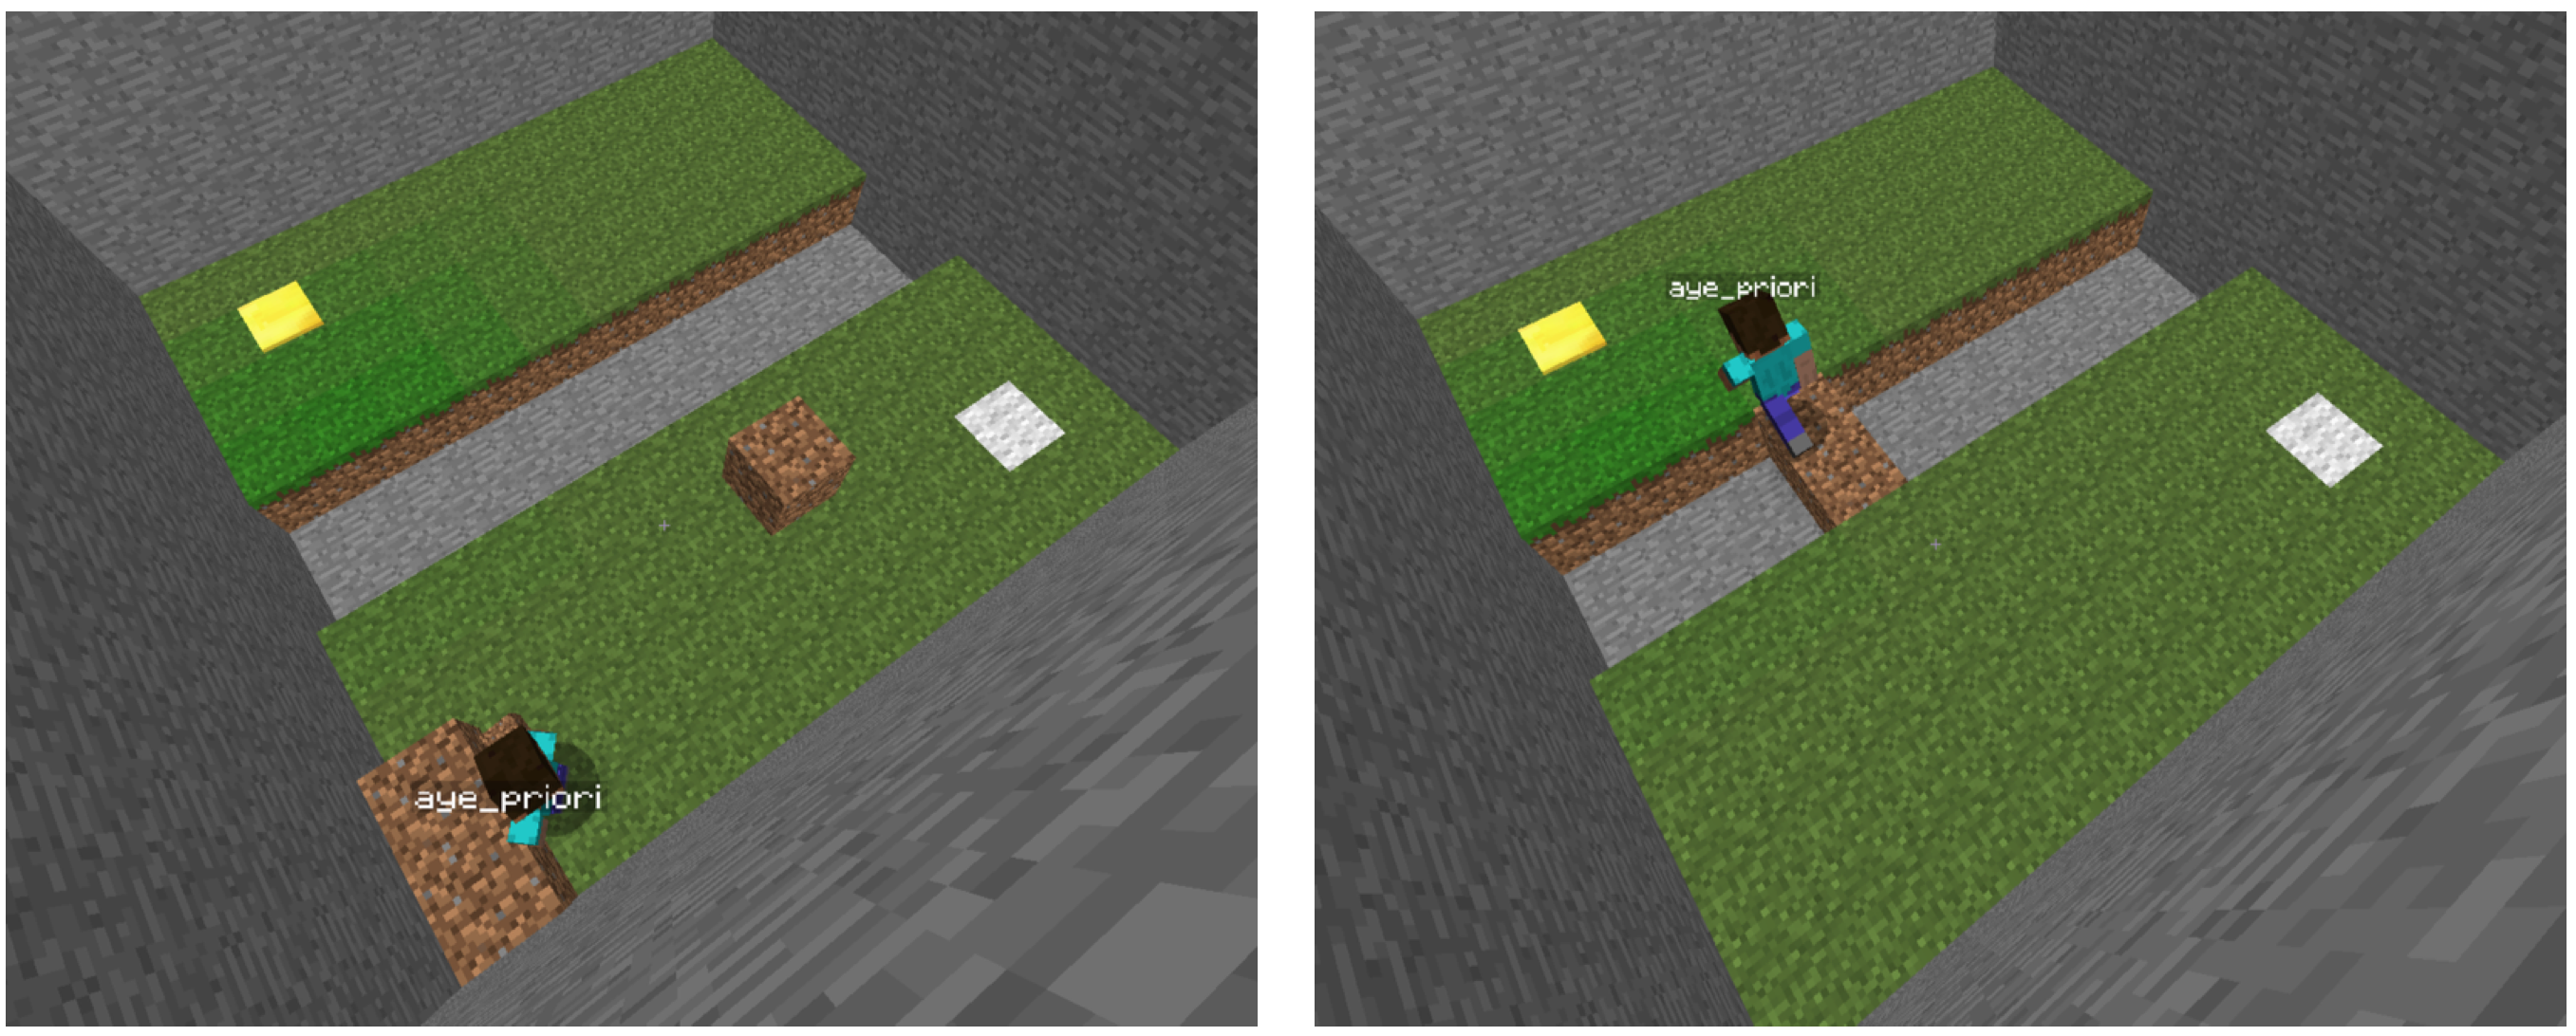
\includegraphics[scale=0.18]{figures/bridgeworld_vi_vs_aff.png}
\subfigure[Start]{
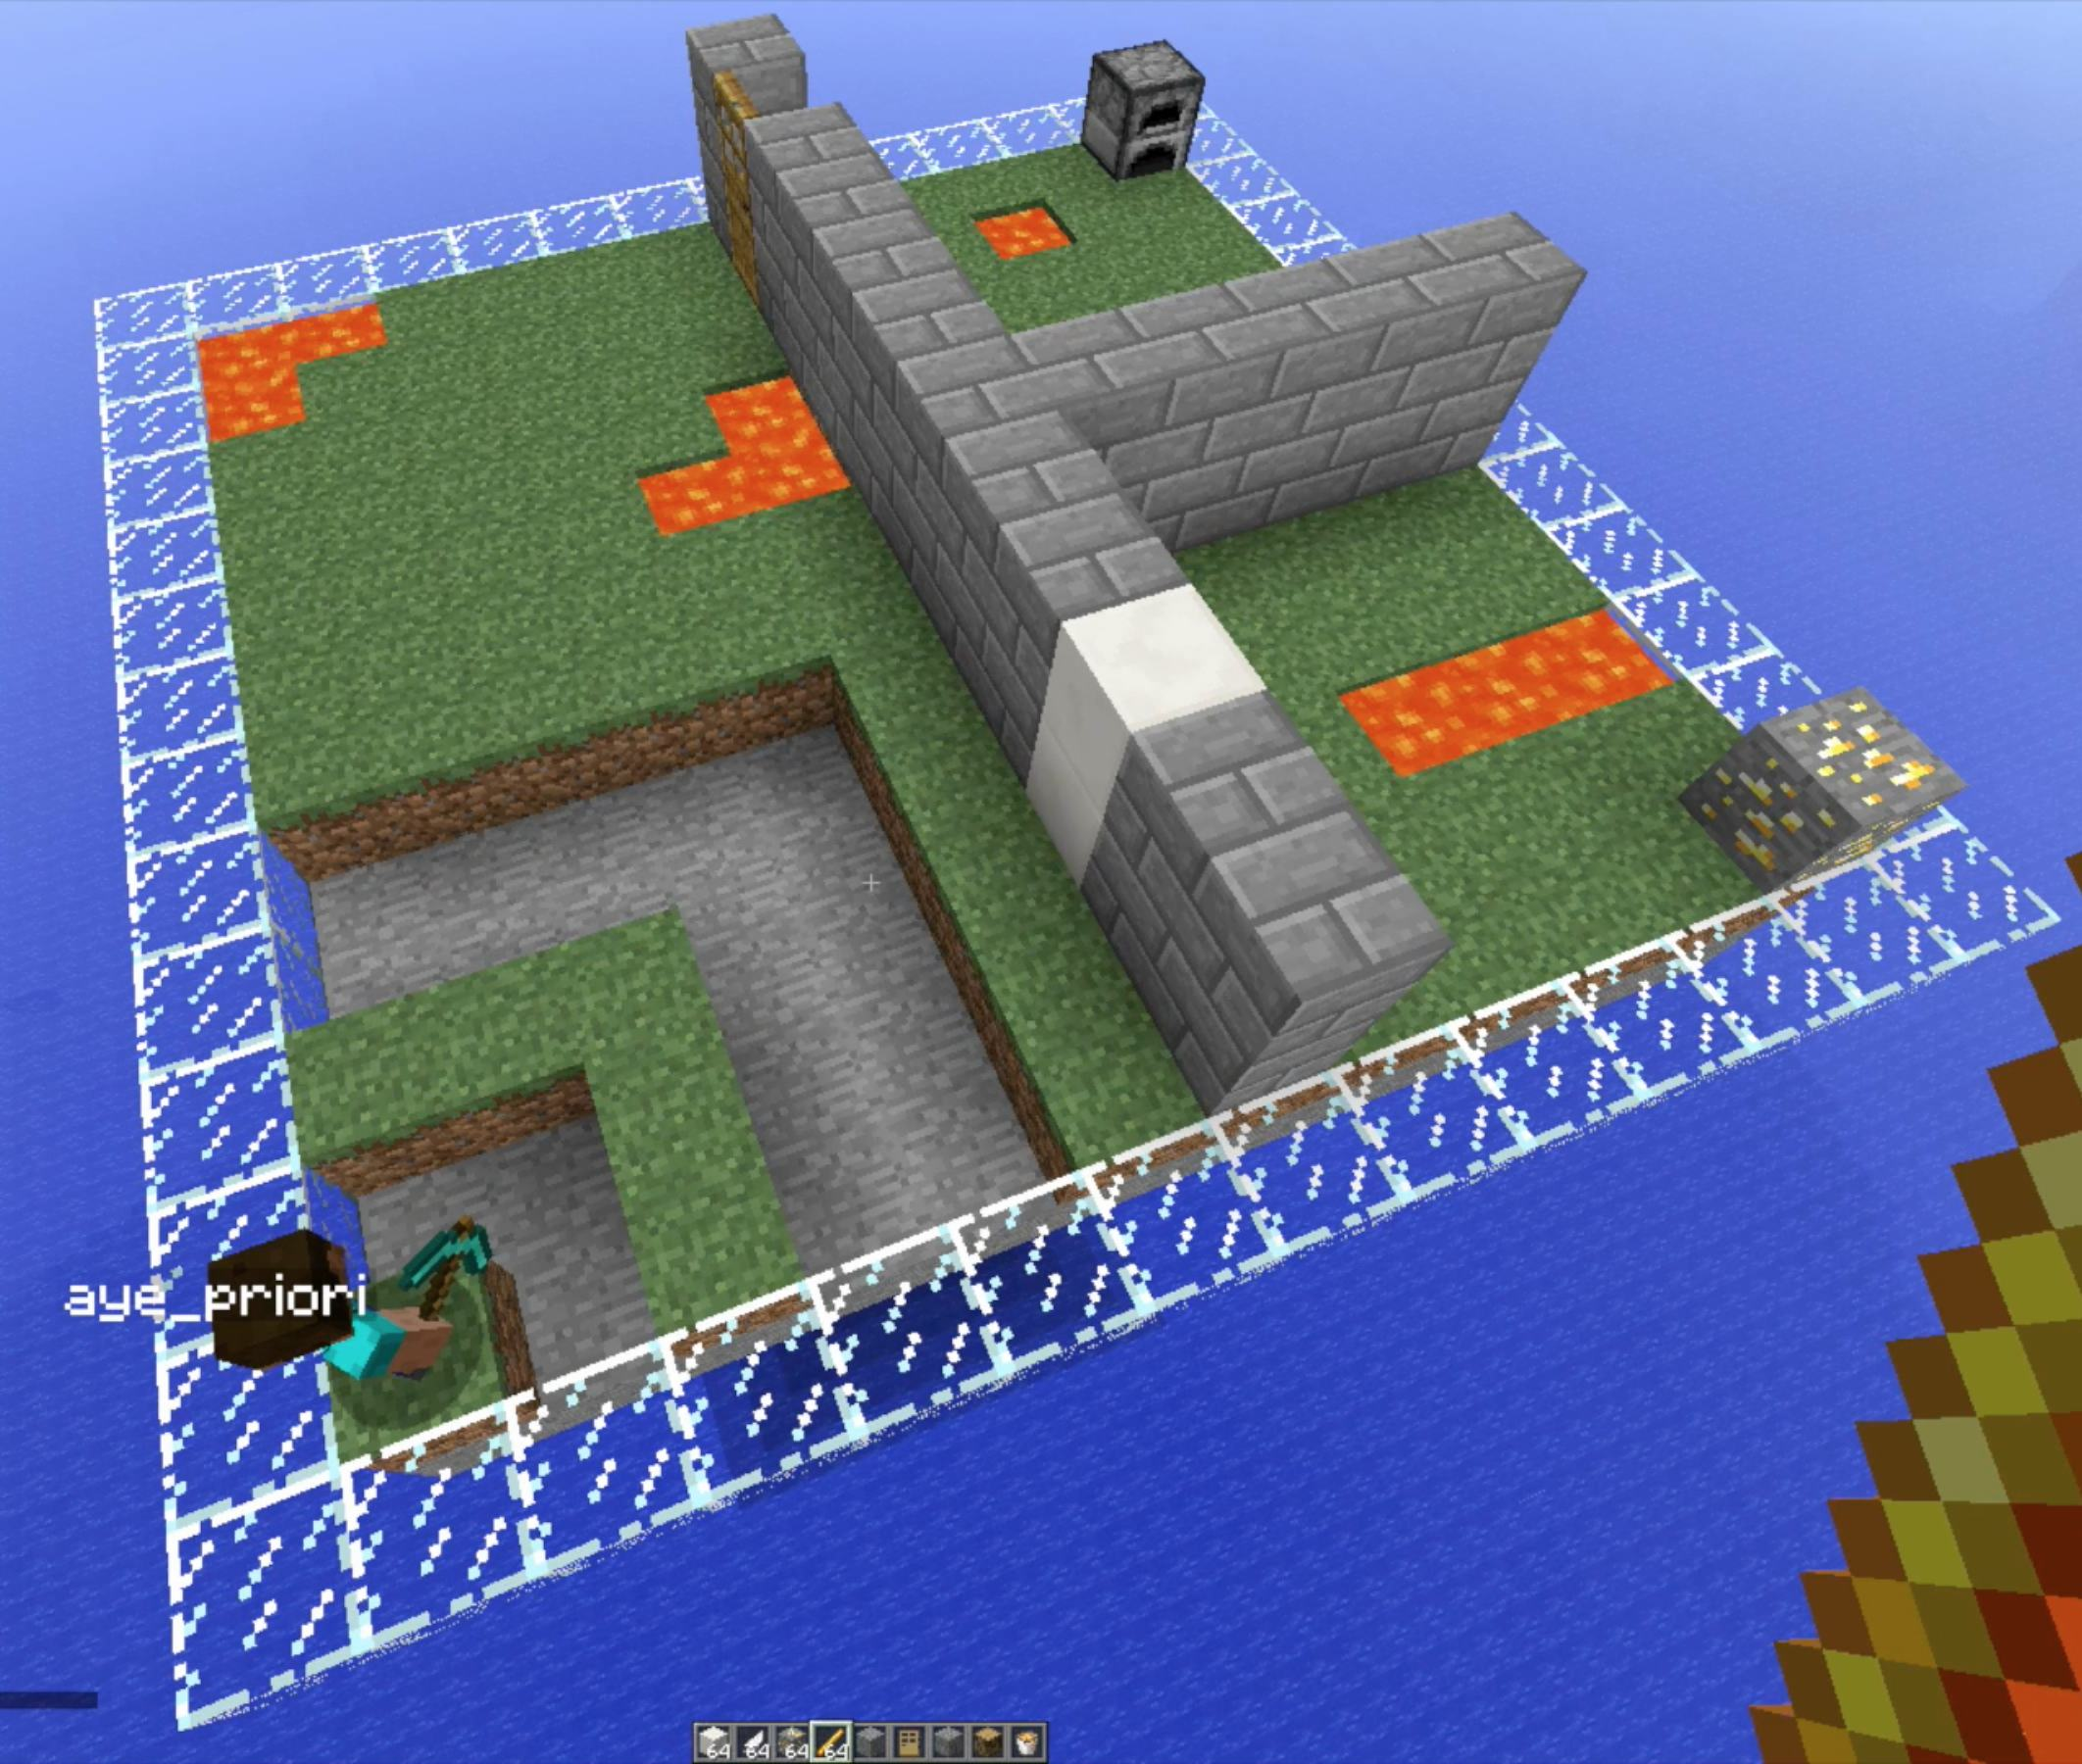
\includegraphics[width=0.24\linewidth]{figures/epicworld_1.png}}%
\subfigure[Destroy Wall]{
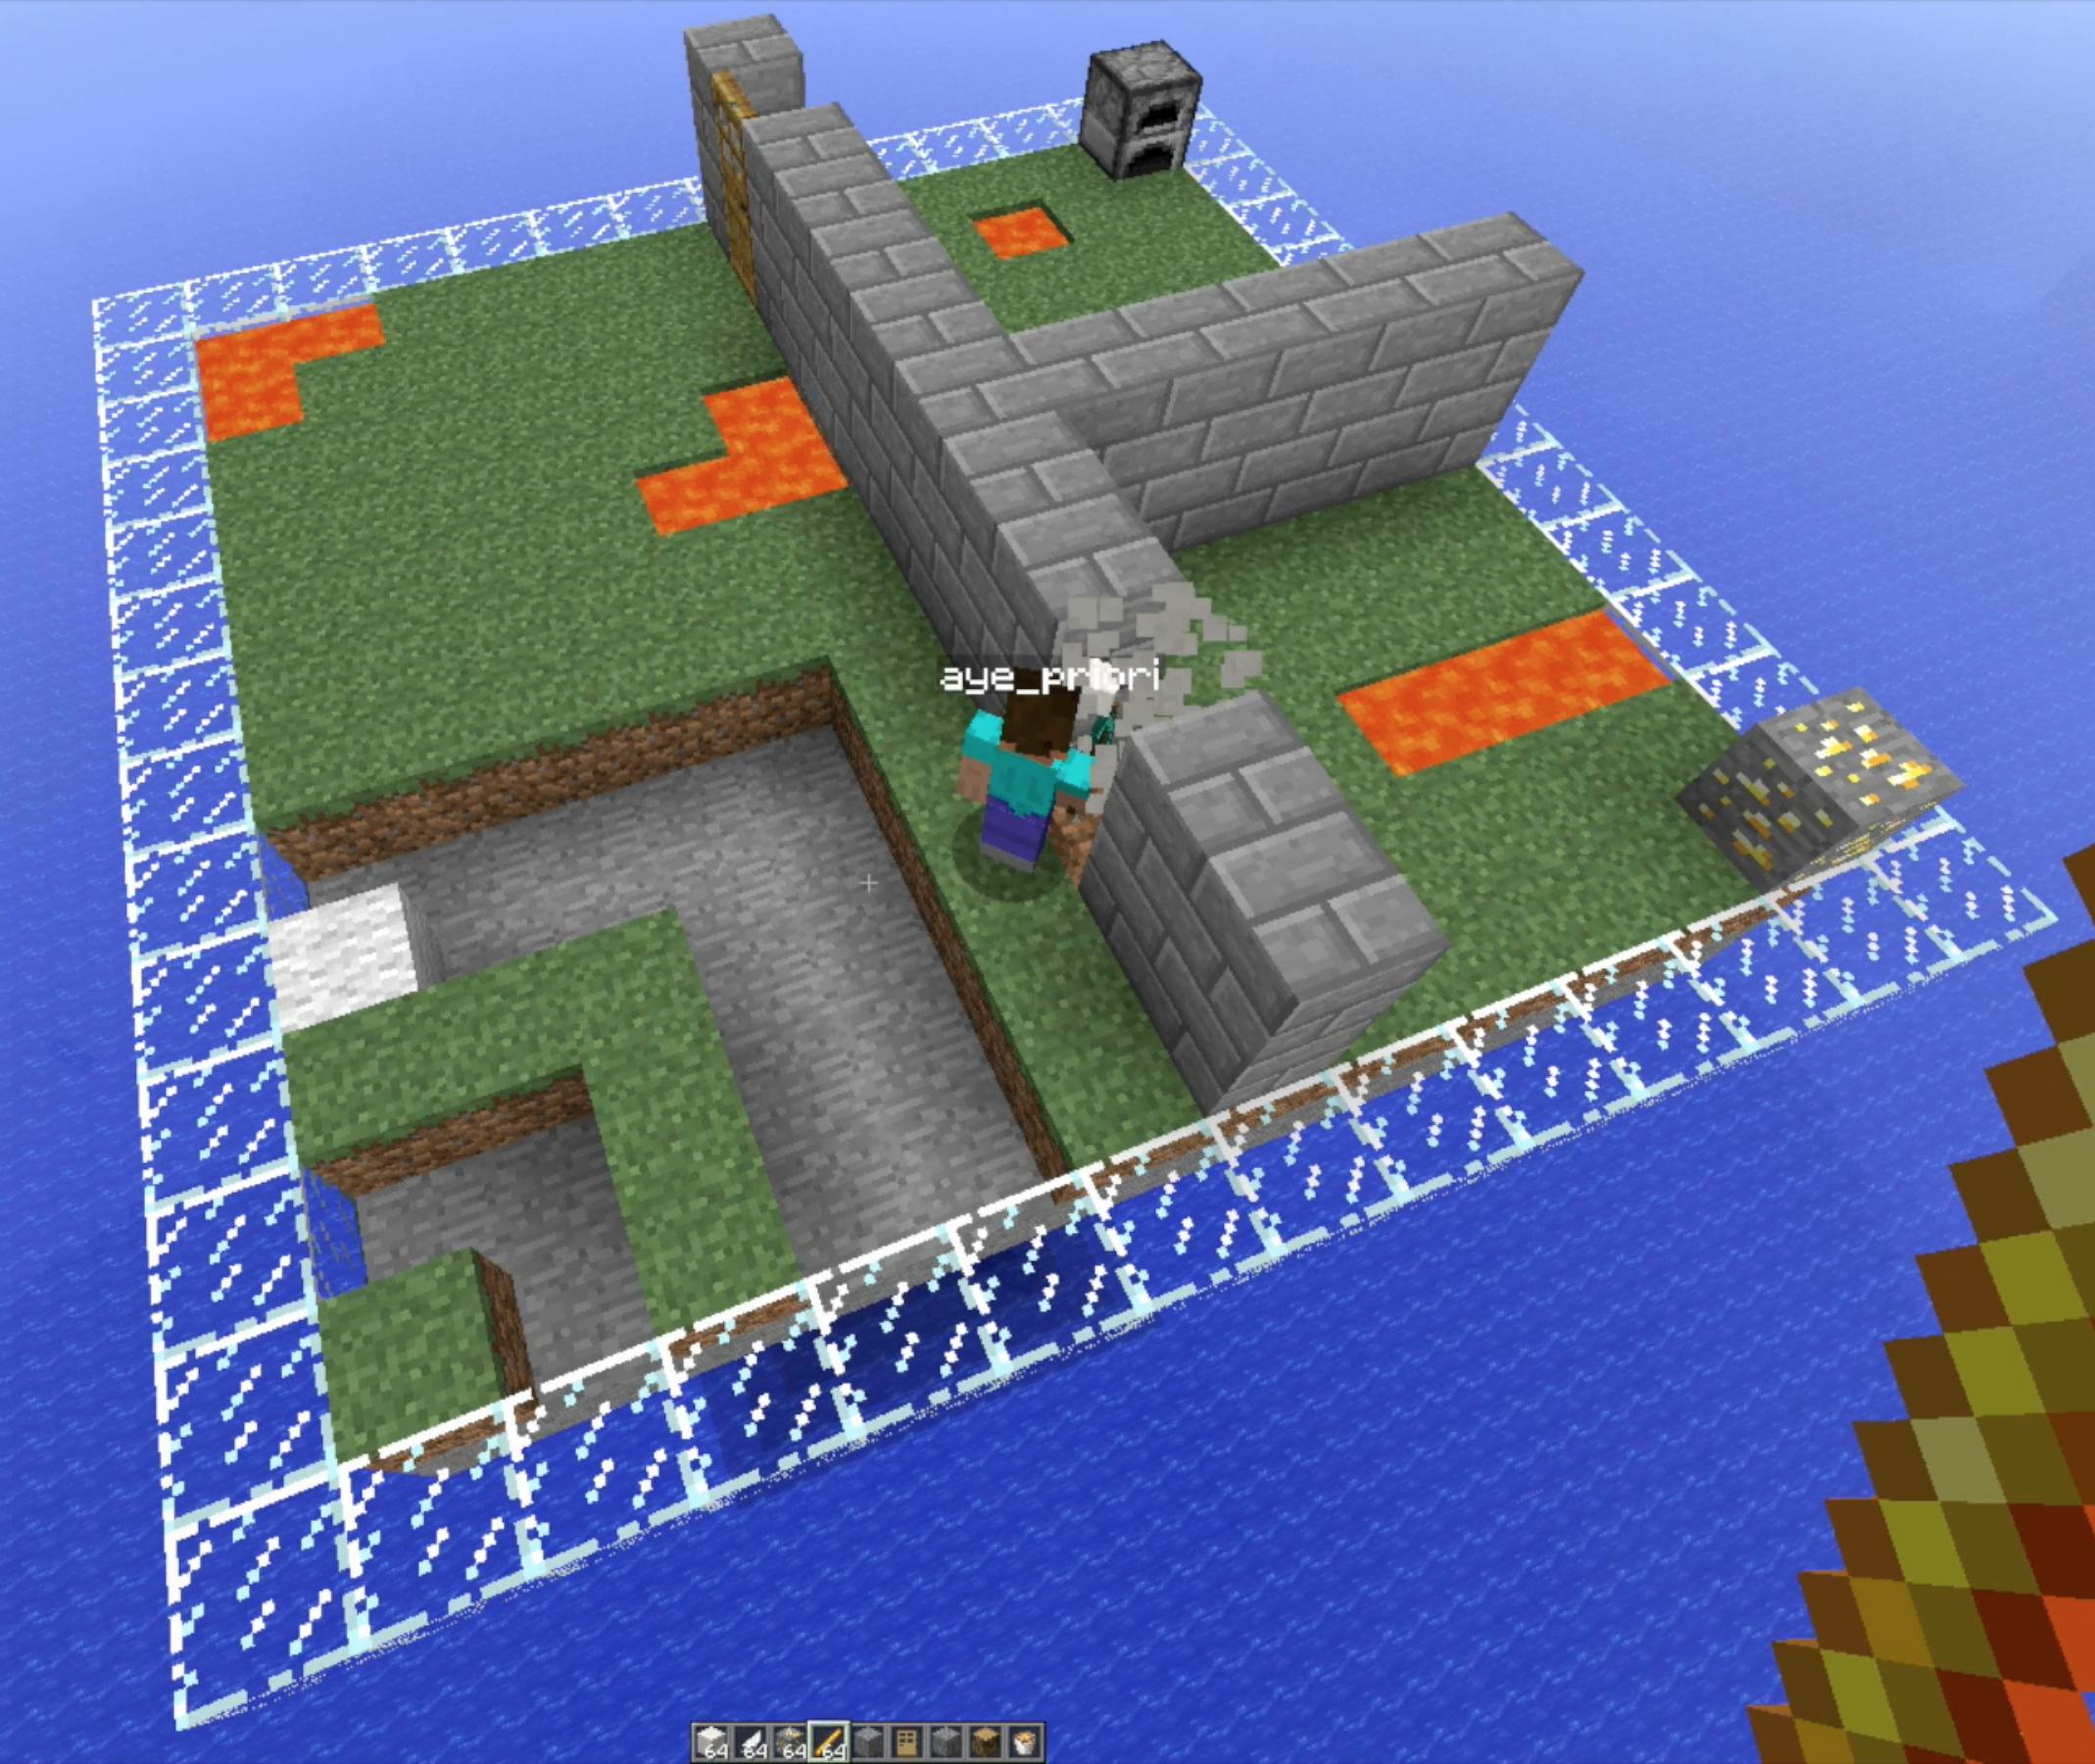
\includegraphics[width=0.24\linewidth]{figures/epicworld_2.png}}%
\subfigure[Collect Ore]{
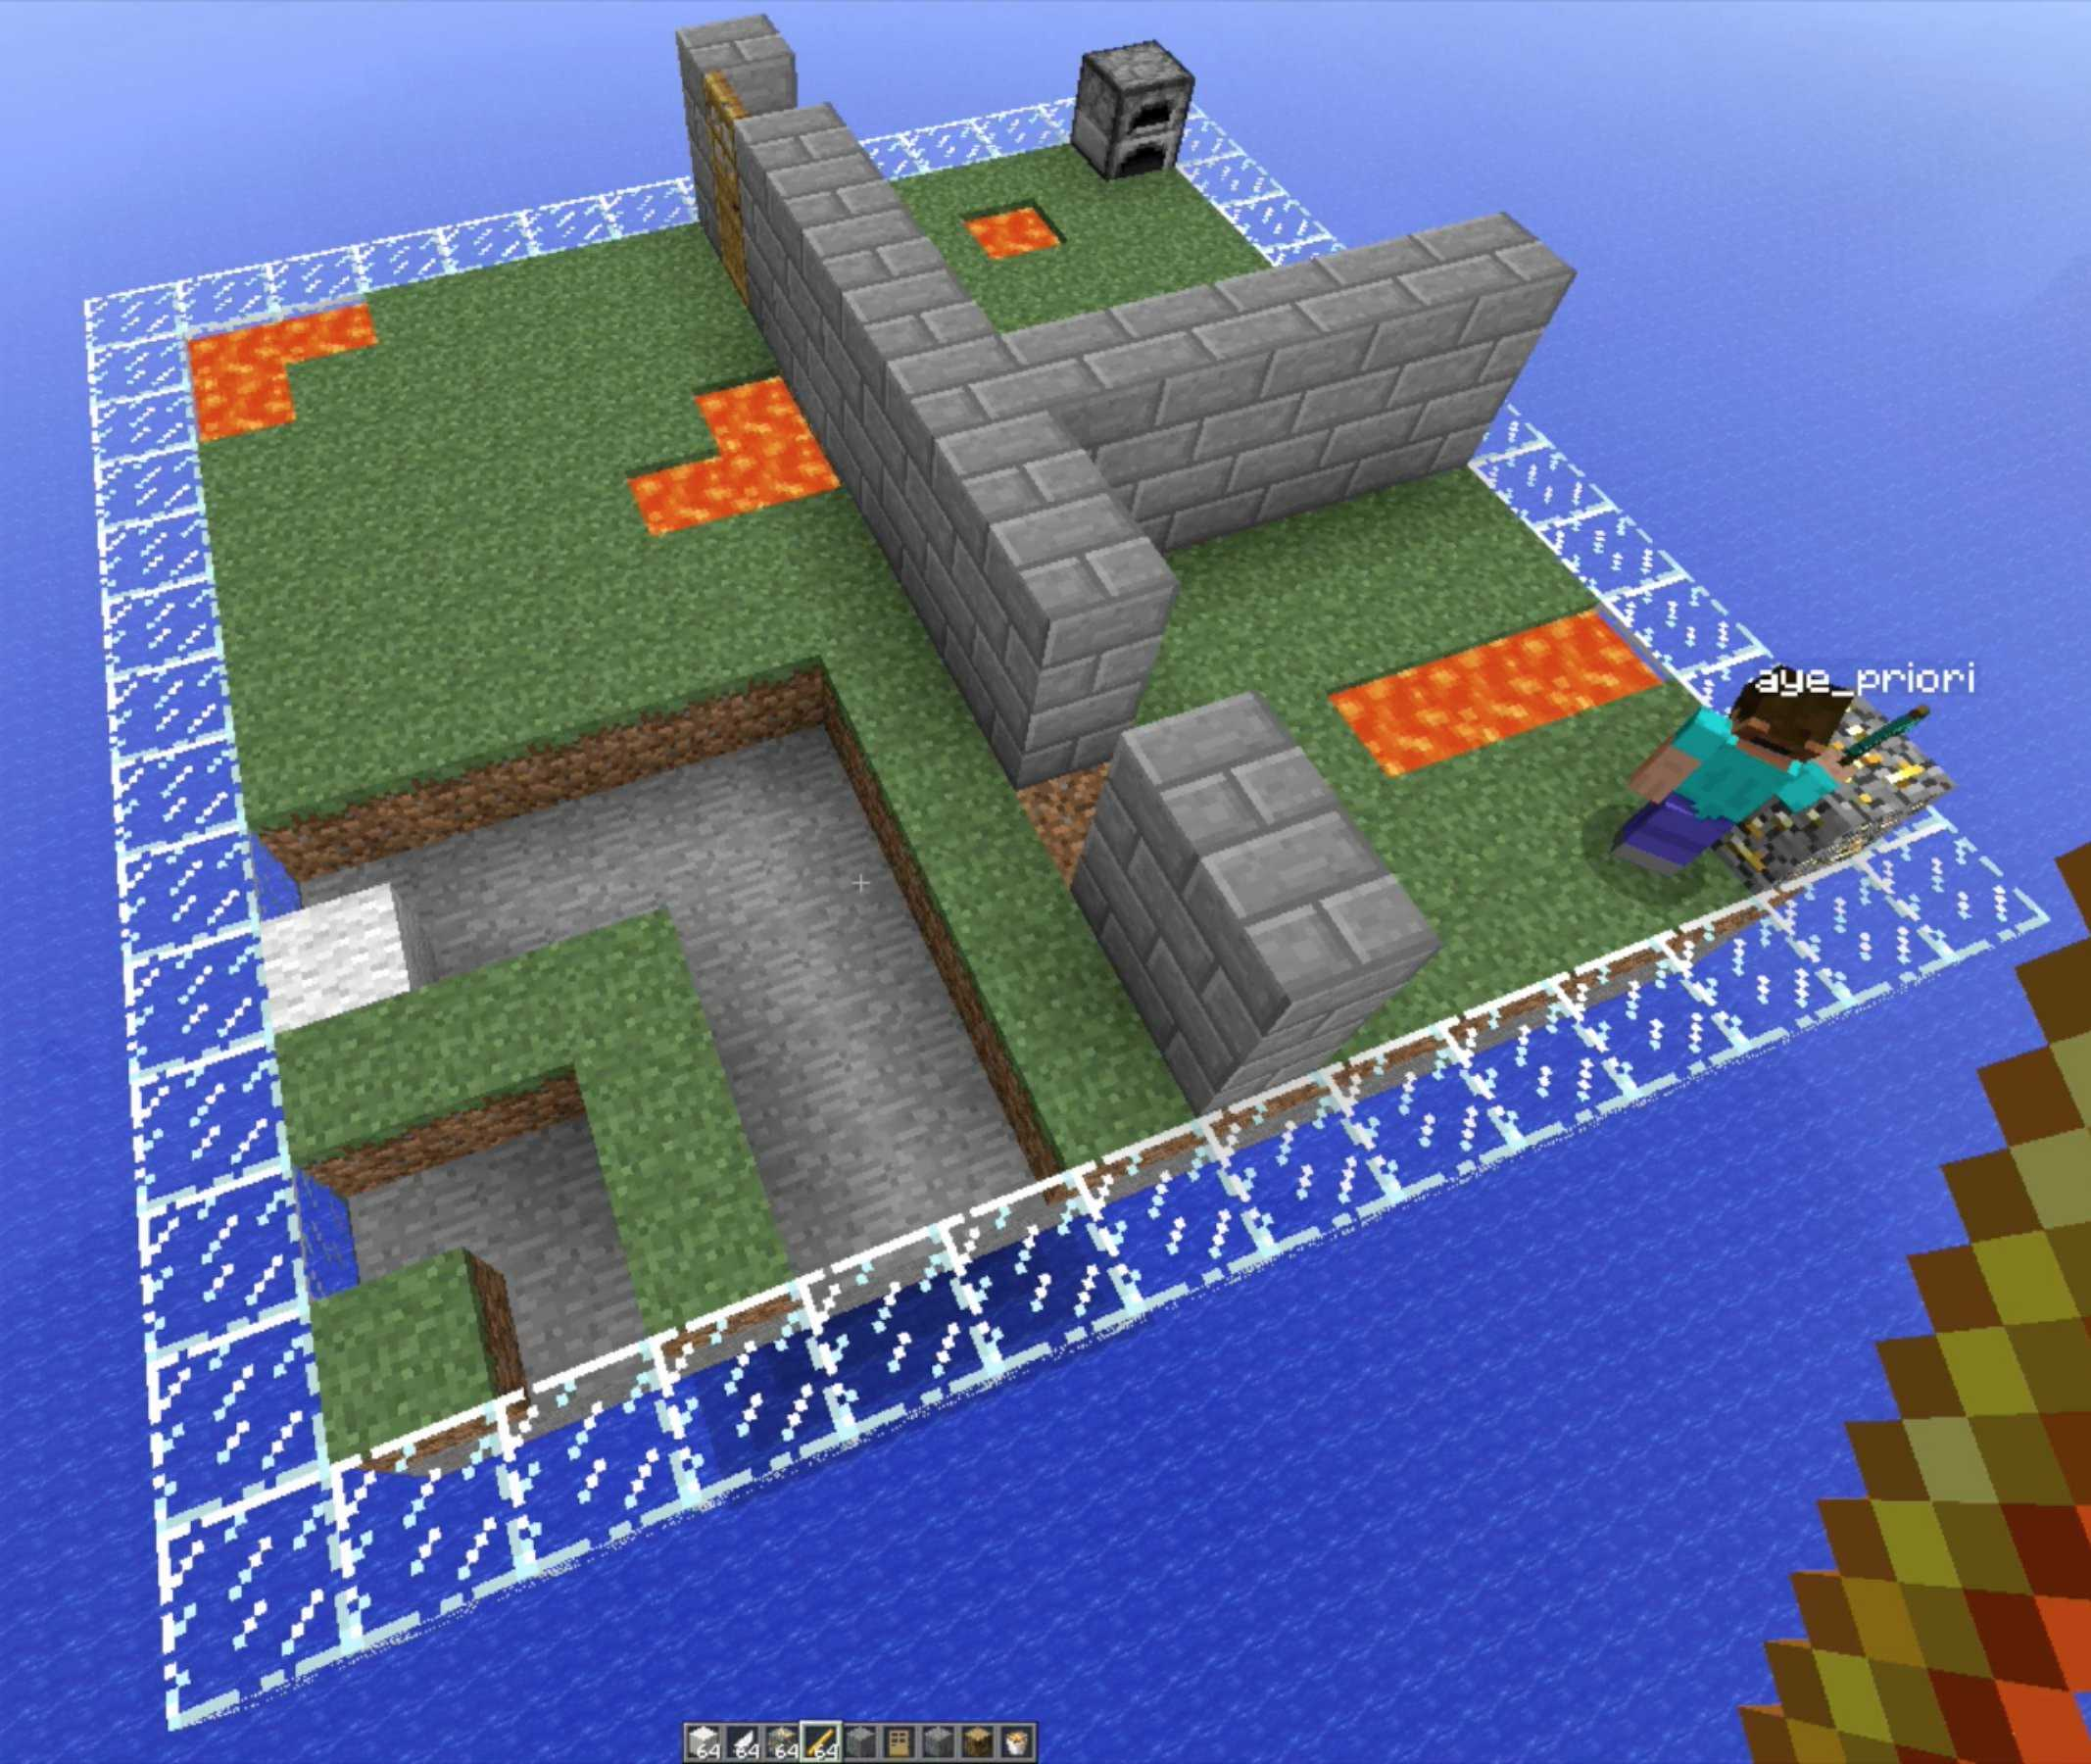
\includegraphics[width=0.24\linewidth]{figures/epicworld_3.png}}%
\subfigure[Smelt Ore]{
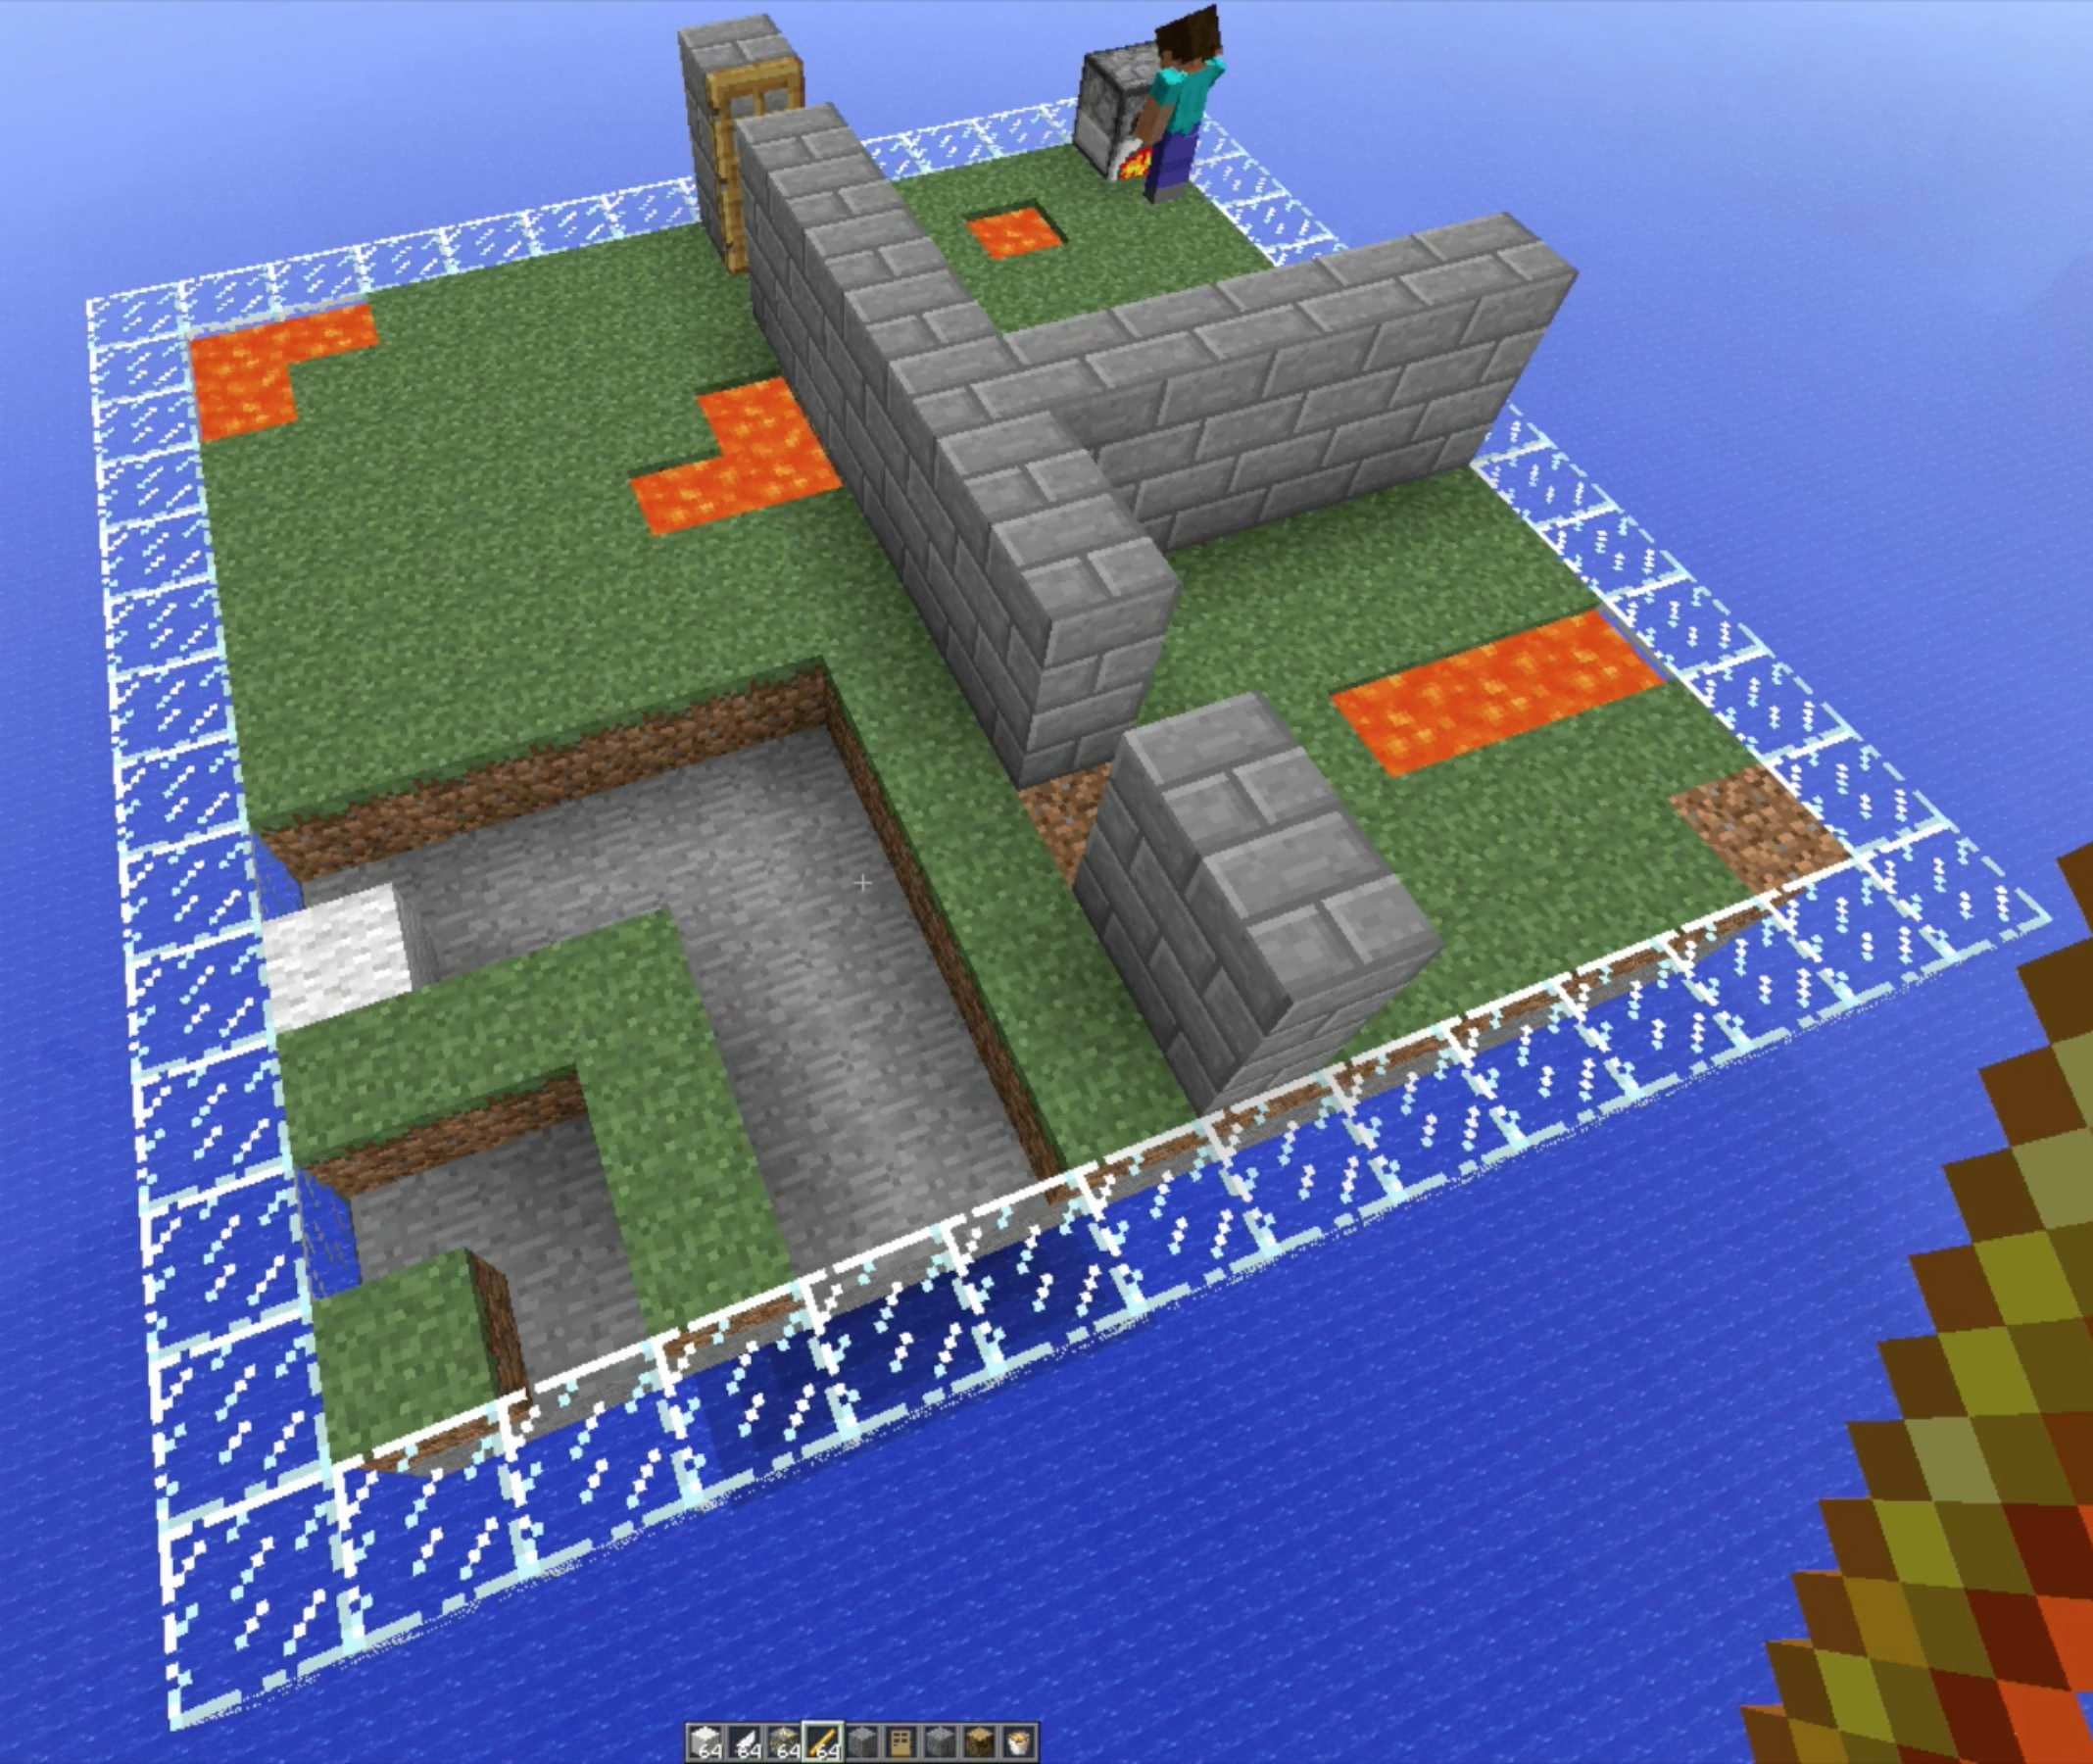
\includegraphics[width=0.24\linewidth]{figures/epicworld_4.png}}%
  \caption{The affordance-aware subgoal planner solving a complicated task: the agent had to jump over trenches,
  place blocks, destroy walls, mine gold, avoid lava, open a door, and finally smelt the gold in order to reach its goal. This task
  was only achievable by the affordance-aware planners.}
  \label{fig:epicworld}
\end{figure*}


One of the most compelling results is the scope of task that affordance-aware planners are capable of solving. With an affordance-aware Subgoal planner (i.e. using an affordance aware RTDP as the low level planner), a Minecraft agent was able to traverse a complicated obstacle course\footnote{A full video of the agent solving this task may be found at: https://vimeo.com/88689171}, as seen in Figure \ref{fig:epicworld}. In this task, the agent had to jump over a trench, build a bridge over another trench, chop down a wall, mine a block of gold, open a door, avoid lava, and finally smelt the gold in a furnace. We have included a video of this task being executed as part of our supplementary materials. In this course, the agent was capable of completing several different types of tasks (subgoals) with a single action space and affordance knowledge base. None of the standard planners even came close to solving this problem - we let them run for several hours before cutting them off (while the affordance-aware subgoal planner found a working policy in under 5 minutes).

\section{Related Work}
In the past, numerous different forms of background knowledge have be used to 
accelerate planning algorithms. In section \ref{sec:subgoals}, subgoal
planning was discussed and in our experimental results, was compared against affordance-aware planning. 
In this section, we discuss the differences between affordance-aware planning and other
forms of background knowledge that have been used to accelerate planning.
Specifically, we discuss heuristics, temporally extended actions, and related action pruning work.
Additionally, we elaborate on other recent attempts of employing Gibson's notion of an affordance 
to the problems of computer science and robotics.


\subsection{Heuristics}
Heuristics in MDPs are used to convey information about the value of a given state or state-action pair with respect to the task being solved and typically take the form of either {\em value function initialization},
or {\em reward shaping}. For planning algorithms that estimate state-value functions, heuristics are often
provided by initializing the value function to values that are good approximations of the true value function. For example, initializing the value function to an admissible close approximation of the optimal value function has been shown to be effective for LAO* and RTDP, because it more greatly biases the states explored by the rollout policy to those important to the optimal policy~\cite{Hansen:1999qf}. Planning algorithms that estimate Q-values instead of the state value function may similarly initialize the Q-values to an approximation of the optimal Q-values. For instance, PROST~\cite{keller2012prost} creates a {\em determinized} version of a stochastic domain (that is, treating each action as if its most likely outcome always occurred), plans a solution in the determinized domain, and then initializes Q-values to the value of each action in the determinized domain.

Reward shaping is an alternative approach to providing heuristics in which the planning algorithm uses a modified version of the reward function that returns larger rewards for state-action pairs that are expected to be useful. Reward shaping differs from value function initialization in that it may not preserve convergence to an optimal policy unless certain properties of the shaped reward are satisfied~\cite{potshap} that also have the effect of making reward shaping equivalent to value function initialization for a large class of planning/learning algorithms~\cite{Wiewiora:2003fk}.

A critical difference between heuristics and affordances is that heuristics are highly dependent on the reward function and state space of the task being solved; therefore, different tasks require different heuristics to be provided, whereas affordances are state independent and transferable between different reward functions. However, if a heuristic can be provided, the combination of heuristics and affordances may even more greatly accelerate planning algorithms than either approach alone.


\subsection{Temporally Extended Actions}

{\em Temporally extended actions} are actions that the agent can
select like any other action of the domain, except executing them
results in multiple primitive actions being executed in
succession. Two common forms of temporally extended actions are {\em
  macro-actions}%~\citep{hauskrecht98}
%   \jmnote{looking at the citaiton you added for macros Stefanie, I think those are still ``options''
%  rather than fixed primitive action sequences. Unfortunatley the term is overloaded a lot.}
  ~and {\em
  options}~\citep{sutton99}. Macro-actions are actions that always
execute the same sequence of primitive actions. Options are defined
with high-level policies that accomplish specific sub tasks. For
instance, when an agent is near a door, the agent can engage the
`door-opening-option-policy', which switches from the standard
high-level planner to running a policy that is hand crafted to open
doors. An option $o$ is defined as follows:

$o\ =\ \langle \pi_0, I_0, \beta_0\rangle$, where:
\begin{align*}
&\pi_0 : (s,a) \rightarrow [0,1] \\
&I_0 : s \rightarrow \{0,1\} \\
&\beta_0 : s \rightarrow [0,1]
\end{align*}

Here, $\pi_0$ represents the {\it option policy}, $I_0$ represents
a precondition, under which the option policy may initiate, and 
$\beta_0$ represent the post condition, which determines which 
states terminate the execution of the option policy.

Although the classic options framework is not generalizable to different state spaces,
creating {\em portable} options is a topic of active research~\citep{konidaris07,konidaris2009efficient,Ravindran03analgebraic,croonenborghs2008learning,andre2002state,konidaris2012transfer}.

Although temporally extended actions are typically used
because they represent action sequences (or sub policies) that are often useful to solving
the current task, they can sometimes have the paradoxical effect
of increasing the planning time because they increase the number of actions that must be explored.
For example, deterministic planning algorithms that successfully make use of macro-actions often avoid the potential increase
in planning time by developing algorithms that restrict the set of macro-actions to a small set that is expected to improve planning time~\citep{Botea:2005kx,Newton:2005vn} or by limiting the use of macro-actions to certain conditions
in the planning algorithms like when the planner reaches heuristic plateaus (areas of the state space in which all successor states have the same heuristic value)~\cite{Coles:2007ys}. Similarly, it has been shown that the inclusion
of even a small subset of unhelpful options can negatively impact planning/learning time~\cite{Jong:2008zr}.

Given the potential for unhelpful temporally extended actions to negatively impact planning time, we believe combing affordances with temporally extended actions
may be especially valuable, because it will restrict the set of temporally extended actions to those
which may actually be useful to a task. In the future, we plan to more directly explore the benefit from combining
these approaches.


%Recently, Konidaris and Barto's ~\citep{konidaris07} 
%expand on the classic options framework and allow for a more portable 
%implementation of options. Still, though, planning with options requires either 
%that we plan in a mixed space of actions {\it and} options (which blows up the 
%size of the search space), or requires that we plan entirely in the space of options. 
%Additionally, providing an agent with an option policy is a difficult task for a human 
%designer (especially if we want an optimal policy, which we do).

\subsection{Action Pruning}
%\jmnote{We should also probably do a search for other MDP action pruning approaches, just to
%make sure we're not missing anything especially important.}

Work that prunes the action space is the most similar to our affordance-aware planning.
%Perhaps the most similar work to ours is Sherstov and Stone's action transfer work~\cite{sherstov2005improving}.
Sherstov and Stone~\cite{sherstov2005improving} considered MDPs with a very large action set and for which the action
set of the optimal policy of a source task could be transferred to a new, but similar, target
task to reduce the learning time required to find the optimal policy in the target task. Since the actions
of the optimal policy of a source task may not include all the actions of the optimal policy
in the target task, source task action bias was reduced by randomly perturbing the value function
of the source task to produce new synthetic tasks. The action set transferred to the target task
was then taken as the union of the actions in the optimal policies for the source task and all the
synthetic tasks generated from it.

A critical difference between our affordance-based action set pruning and this action transfer
work is that affordances prune away actions on a state by state basis. Therefore, affordance aware
planners are significantly more flexible as they move throughout a state space, as certain actions
are useful for a given planning task in general, but not in specific subspaces of the statespace. Further,
with lifted goal descriptions, affordances may be attached to Subgoal planning for a huge
benefit in planning tasks where complete subgoal knowledge is known (or may be inferred).

Rosman and Ramamoorthy~\cite{rosman2012good} provide a method for learning action priors over a set of related tasks. Specifically, a Dirichlet distribution over actions was computed by extracting the frequency that each action was optimal in each state for each previously solved task. On a novel task learned with Q-learning, a variant of an $\epsilon$-greedy policy was followed in which the agent selcted a random action according to the Dirichlet distribution and $\epsilon$ fraction of the time, and the action with the max Q-value the rest of the time. To avoid dependence on a specific state space, the a Dirichlet distribtuion was created for each observation-action pair (where the observations were task indepdent) instead of each state-action pair.

There are a few limitations of the actions priors work that affordance-aware planning does not possess: (1) the action priors can only be used with planning/learning algorithms that work well with an $\epsilon$-greedy rollout policy; (2) the priors are only utilized for fraction $\epsilon$ of the time steps, which is typically quite small; and (3) as variance in tasks explored increases, the priors will become more uniform. In contrast, affordance-aware planning can be used in a wide range of planning algorithms, benefits from the pruned action set in every time step, and the affordance defined lifted goal-description and enables higher-level resoning such as subgoal planning. However, in the future, the action set each affordance defines could be learned using a similar approach.

\dnote{I also found several other action pruning papers we may want to talk about (see comments for list)}
% Mausam, Weld (2008): http://www.aaai.org/Papers/JAIR/Vol31/JAIR-3102.pdf
% Raghavan, Khardon, Fern, Tadepalli: http://papers.nips.cc/paper/5143-symbolic-opportunistic-policy-iteration-for-factored-action-mdps.pdf
% Oliehoek, Spaan: http://citeseerx.ist.psu.edu/viewdoc/download?doi=10.1.1.387.1488&rep=rep1&type=pdf}


\subsection{Affordances}
As mentioned before, there have been plenty of other successful attempts at defining Affordances, though as expected, each respective definition
has its own quirks depending on the desired application.

% Steedman
Mark Steedman has done quite a bit of work in formalizing affordances, specifically aimed at resolving the Frame Problem and integration with deterministic symbolic planning, such as Metric-FF. (cite).

% Saxena
Ashutosh Saxena and Hema Koppula recently developed an inference algorithm that enables a robotic agent to anticipate a human's actions based on the robots perceived affordances in its current environment. 

% Gorniak/Roy
Peter Gorniak and Deb Roy have jointly done a lot of work with what they call the Affordance-Based-Concept (cite). They are interested
in using the perception of affordances as a means of determining the set of possible interactions an agent may engage with in a given context.
Gorniak's doctoral dissertation developed this theory, and they have since done a variety of projects leveraging it. (expand).

\dnote{There are many other affordance/robotics projects I've come across that we could consider including (commented out currently, see .tex file)}
%Others:
%\begin{itemize}
%\item Learning Visual Object Categories for Robot Affordance Prediction 
%\item Learning grasping affordances from local visual descriptors
%\item Gibsonian Affordances for Roboticists
%\item To Afford or Not to Afford: A New Formalization of Affordances Toward Affordance-Based Robot Control
%\item Learning Object Affordances: From Sensory--Motor Coordination to Imitation
%\item Behavior-Grounded Representation of Tool Affordances
%\item Affordance-based imitation learning in robots
%\item Traversability: A Case Study for Learning and Perceiving Affordances in Robots
%\item Toward learning the binding affordances of objects: A behavior-grounded approach
%\item Case studies of applying Gibson's ecological approach to mobile robots
%\item Towards Affordance-based Robot Control
%\item Localizing Grasp Affordances in 3-D Points Clouds Using Taubin Quadric Fitting
%\end{itemize}


\section{CONCLUSION}

We proposed a novel approach to representing knowledge in terms of
{\em affordances}~\citep{gibson77} that allows an agent to efficiently
prune its action space based on domain knowledge. This led to the 
proposal of affordance-aware planners, which improve on classic planners
by providing a significant reduction in the number of state/action pairs the
agent needs to evaluate in order to act optimally. We demonstrated the efficacy 
as well as the portability of the affordance model by comparing standard paradigm
planners to their affordance-aware equivalents in a series of planning tasks in the Minecraft
domain.

In the future, we hope to introduce a more robust inference system around pruning actions, such that
the agent not only prunes away {\it useless} actions, but also prioritizes between
{\it great} actions, and {\it mediocre} ones. This also lends itself nicely for applying
machine learning techniques to learn affordances directly, which would 
overcome the fact that a human designer must currently hand craft affordance knowledge bases.
Further, we foresee extensions in natural language processing and information
extraction, in which affordances may be inferred via text or from dialogue with a human partner.
This promises extensions in which a robotic agent receives aid from a human partner through natural language
dialogue; the agent may ask for help when it is stuck and
receive affordance or subgoal {\it hints} from a human companion. Lastly, we consider applications to a variety of other planning
strategies, including making A* affordance aware for use in a robotic-cooking companion, and enhancing POMDPs\footnote{a classical extension of the MDP in which the agent must make decisions with respect to a distribution over a {\it belief} state,
as opposed to knowing precisely what state it is in at all times} with affordances, directed at applications to robotic care-giver companions.

\bibliographystyle{plainnat}
\bibliography{main}  


\end{document}
